\documentclass[twocolumn]{article}
%\usepackage[spanish]{babel}
\usepackage[utf8]{inputenc}
\usepackage{amsmath}
\usepackage{natbib}
\usepackage{microtype}
\usepackage{etoolbox}
\usepackage{amssymb}
\usepackage{graphicx}
\usepackage{lipsum}
\usepackage{fancyhdr}
\usepackage{abstract}
\usepackage{geometry}
\usepackage{booktabs}
\usepackage{url}

% Ubicación de los gráficos 
\graphicspath{ {imagenes/} }

% DEFINIR LOS COMANDOS QUE FALTAN
\providecommand{\apjs}{ApJ Suppl. Ser.}
\providecommand{\aj}{Astron. J.}
\providecommand{\apj}{Astrophys. J.}
\providecommand{\apjl}{Astrophys. J. Lett.}
\providecommand{\aap}{Astron. Astrophys.}
\providecommand{\mnras}{Mon. Not. R. Astron. Soc.}
\providecommand{\pasa}{Publications of the Astronomical Society of Australia}

% Configuración de página
\geometry{a4paper, margin=1in}

% Configuración de encabezados
\pagestyle{fancy}
\fancyhf{}
\fancyhead[L]{\small Morfología y propiedades de galaxias en Sloan}
\fancyhead[R]{\small \thepage}
\fancyfoot[C]{\footnotesize Astronomía Extragaláctica - 2025 - J.M. Puddu}

% Configuración del abstract para una columna
\renewcommand{\abstractname}{Resumen}
\setlength{\absleftindent}{0pt}
\setlength{\absrightindent}{0pt}

\title{Morfología y propiedades de galaxias en Sloan Digital Sky Survey}
\author{J.M. Puddu \\ FAMAF - Universidad Nacional de Córdoba - Argentina}
\date{\today}

\begin{document}

\twocolumn[
\begin{@twocolumnfalse}
    \maketitle
    \begin{abstract}
        \noindent Este trabajo presenta un análisis estadístico de la morfología y propiedades de galaxias utilizando datos del Sloan Digital Sky Survey (SDSS). Se estudian características visuales y espectroscópicas de una muestra de 20,000 galaxias con el objetivo de comprender los procesos físicos subyacentes y extraer información relevante para estudios extragalácticos. Se analizan parámetros morfológicos, distribución de colores, relaciones tamaño-luminosidad y diagramas color-magnitud, identificando correlaciones entre las propiedades estructurales y poblaciones estelares.
        
        \vspace{0.5em}
        \noindent\textbf{Palabras clave}: Galaxias, Morfología, SDSS, Astronomía extragaláctica, Análisis estadístico
    \end{abstract}
    \vspace{2em}
\end{@twocolumnfalse}
]

\section{Introducción}

Para inferir los procesos físicos que ocurren dentro de una galaxia es necesario comprender en profundidad las características ``visuales'' que esta presenta. Al observarlas, ya sea de forma directa o utilizando espectroscopía, obtenemos información de manera indirecta sobre su estructura y composición.

Los catálogos o \textit{surveys} son los encargados de extraer la versión más primitiva de esta información, cada uno con su propio criterio. Este trabajo tiene como objetivo comprender estas características fundamentales y cómo obtener información relevante sobre las galaxias en general a partir de ellas.

\subsection{Sloan Digital Sky Survey (SDSS)}

El Sloan Digital Sky Survey (SDSS) es uno de los catálogos más relevantes y con mayor trayectoria en el área. Utiliza un telescopio de 2.5 metros de diámetro ubicado en el Observatorio de Apache Point en Sunspot, Nuevo México, a 2788 metros sobre el nivel del mar. El survey cuenta con 19 \textit{Data Releases} (DR) y cubre regiones específicas del cielo (Figura \ref{fig:sky_araña}).

SDSS trabaja con cinco filtros: $u$, $g$, $r$, $i$, $z$. Es común caracterizar las galaxias según sus propiedades en el filtro $r$, ya que se asemeja más a la región visible del espectro electromagnético.

En este trabajo se utiliza una muestra de 20,000 galaxias del catálogo DR17 de SDSS \citep{2022ApJS..259...35A}, sometida a una limpieza preliminar y analizada mediante datos fotométricos y espectroscópicos.

\subsection{Muestras de galaxias}

El propósito de este trabajo es estudiar las propiedades generales de las galaxias utilizando un conjunto de muestra grande y representativo. Considerando la expansión del universo y su efecto en la radiación recibida, se definen dos tipos de muestras:

\begin{itemize}
    \item \textbf{Muestras completas por flujo}: Seleccionadas por brillo aparente
    \item \textbf{Muestras completas por volumen}: Seleccionadas por distancia
\end{itemize}

Posteriormente se detallará en qué categoría se encuentra nuestra muestra de datos.

\section{Marco teórico}

Esta sección presenta una versión resumida de los conceptos y características utilizados en este trabajo, enfocándose en las definiciones empleadas por SDSS.

\subsection{Morfología de galaxias}

La clasificación morfológica desarrollada por Hubble \citep{1926ApJ....64..321H} categoriza las galaxias en cuatro tipos principales:

\begin{itemize}
    \item \textbf{Galaxias elípticas (E)} presentan isofotas\footnote{Las isofotas son contornos a lo largo de los cuales el brillo superficial de una fuente es constante. Si el perfil de luz de una galaxia es elíptico, entonces sus isofotas son elipses.} casi elípticas sin estructura claramente definida. Se subdividen según su elipticidad $\epsilon = 1 - b/a$, donde $a$ y $b$ denotan los semiejes mayor y menor, respectivamente. El rango de elipticidad es $0 \lesssim \epsilon \lesssim 0.7$. La notación En clasifica las elípticas con $n = 10(1 - b/a)$; una galaxia E4 tiene relación de ejes $b/a = 0.6$, y las E0 tienen isofotas circulares. Presentan baja tasa de formación estelar y población estelar vieja.

    \item \textbf{Galaxias espirales} consisten en un disco con estructura de brazos espirales y bulbo central. Se dividen en espirales normales (S) y barradas (SB). La secuencia (a, ab, b, bc, c, cd, d) ordena según la relación de brillo bulbo-disco. Presentan población estelar compleja: discos con población joven y formación estelar, halos con estrellas viejas.

    \item \textbf{Galaxias irregulares (Irr)} muestran estructura regular débil (Irr I) o ausente (Irr II). Presentan alta tasa de formación estelar e incluyen galaxias en interacción.

    \item \textbf{Galaxias S0 (lenticulares)} son transición entre elípticas y espirales, con bulbo y disco sin brazos espirales definidos.
\end{itemize}

La nomenclatura ``tempranas'' (elípticas, S0) y ``tardías'' (espirales, irregulares) se mantiene por convención histórica, aunque no refleja secuencia evolutiva.

\subsection{Tamaño de galaxias}

SDSS define el tamaño galáctico como el radio que contiene cierto porcentaje del brillo total. Los parámetros típicos son $r_{50}$ (radio que contiene el 50\% del flujo) y $r_{90}$ (90\% del flujo).

\subsubsection{Parámetro de concentración}

Define cuán concentrada es una galaxia:
\begin{equation}
    C = \frac{r_{50}}{r_{90}}
\end{equation}

\subsection{Magnitudes}

\subsubsection{Magnitud model}

Se ajustan dos modelos de distribución de brillo:
\begin{itemize}
    \item Perfil de De Vaucouleurs \citep{1948AnAp...11..247D}: 
    \begin{equation}
        I(r) = I_0 e^{-7.67 [(r/r_e)^{1/4}]}
    \end{equation}
    \item Perfil exponencial \citep{1970ApJ...160..811F}:
    \begin{equation}
        I(r) = I_0 e^{-1.68r/r_e}
    \end{equation}
\end{itemize}

La magnitud model se calcula mediante la ley de Pogson:
\begin{equation}
    m_{\text{model}} = 22.5 - 2.5 \log_{10}(f)
\end{equation}

\subsubsection{Magnitud Petrosiana}

El sistema Petrosiano \citep{Petrosian1976} mide flujos dentro de una apertura circular cuyo radio define la forma del perfil de luz promediado azimutalmente. La razón Petrosiana $R_P$ a radio $r$ es:
\begin{equation}
    R_P(r) = \frac{I_{\text{anillo}}(r)}{I_{\text{promedio}}(r)}
\end{equation}

El radio Petrosiano $r_P$ es donde $R_P(r_P) = 0.2$. El flujo Petrosiano se define dentro de $2r_P$, asegurando consistencia en medidas de color.

\subsubsection{Parámetro fracDeV}

Las magnitudes modelo compuestas combinan ambos perfiles:
\begin{equation}
    F_{\text{composite}} = \text{fracDeV} \cdot F_{\text{deV}} + (1 - \text{fracDeV}) \cdot F_{\text{exp}}
\end{equation}

El parámetro fracDeV cuantifica cuánto se asemeja el perfil al de De Vaucouleurs. En este trabajo: $\text{fracDeV} \leq 0.2$ indica disco prominente, $\text{fracDeV} \geq 0.8$ indica bulgo prominente.

\subsection{Brillo superficial}

Define la cantidad de flujo por unidad de superficie recibido de un objeto. Para galaxias, proporciona información sobre la distribución espacial de la luz \citep{2005PASA...22..118G}.

\section{Datos y metodología}

\subsection{Selección de la muestra}

Se descargaron 20,000 galaxias usando CasJobs, seleccionando columnas de las tablas Galaxy y SpecObj con los límites:
\begin{itemize}
    \item Redshift: $0.02 < z < 0.05$
    \item Magnitud Petrosiana $r$: $14 < m_r < 18$ (corregida por extinción)
\end{itemize}

Las restricciones de magnitud aseguran:
\begin{itemize}
    \item Completitud espectroscópica hasta $m_r \sim 17.77$
    \item Evitar saturación en galaxias muy brillantes ($m_r < 14$)
\end{itemize}

\subsection{Caracterización de la muestra}

La Figura \ref{fig:araña} muestra la distribución uniforme en el cielo. La Figura \ref{fig:hist_z} presenta la distribución de redshift, mostrando un pico alrededor de $z \sim 0.03$.

La Figura \ref{fig:completo_flujo} confirma que la muestra es completa por flujo, con distribución uniforme en el rango de magnitudes.

\begin{figure}[ht]
    \centering
    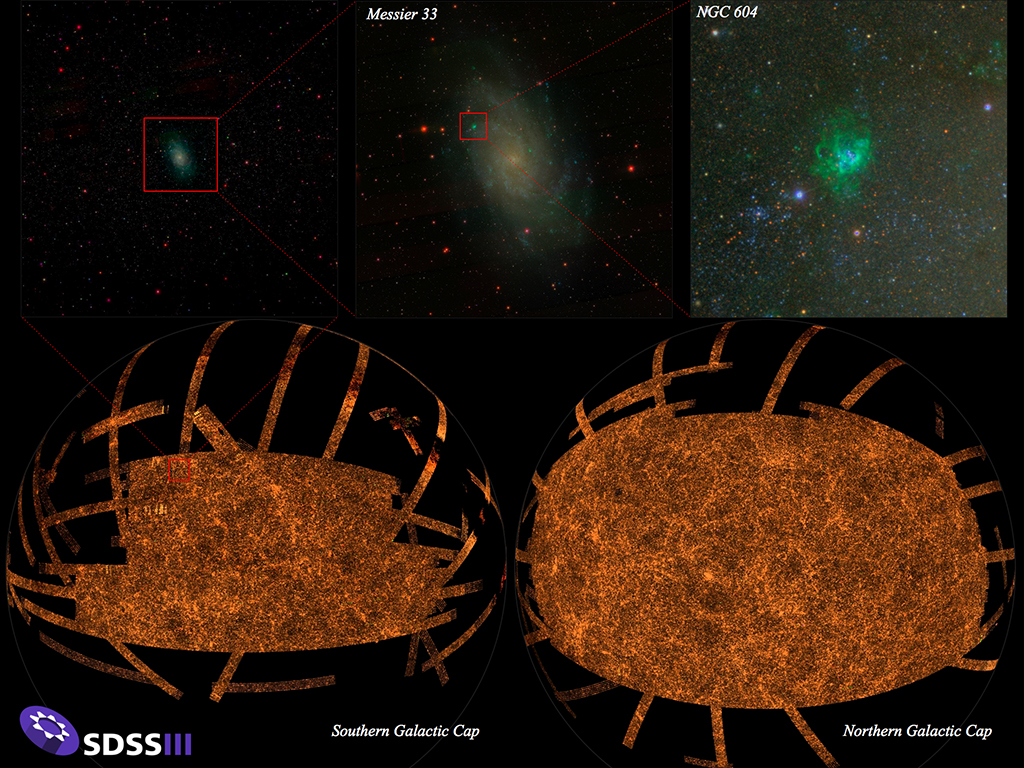
\includegraphics[width=\linewidth]{orangespider-smaller.jpg}
    \caption{Regiones del cielo cubiertas por el catálogo SDSS.}
    \label{fig:sky_araña}
\end{figure}

\begin{figure}[ht]
    \centering
    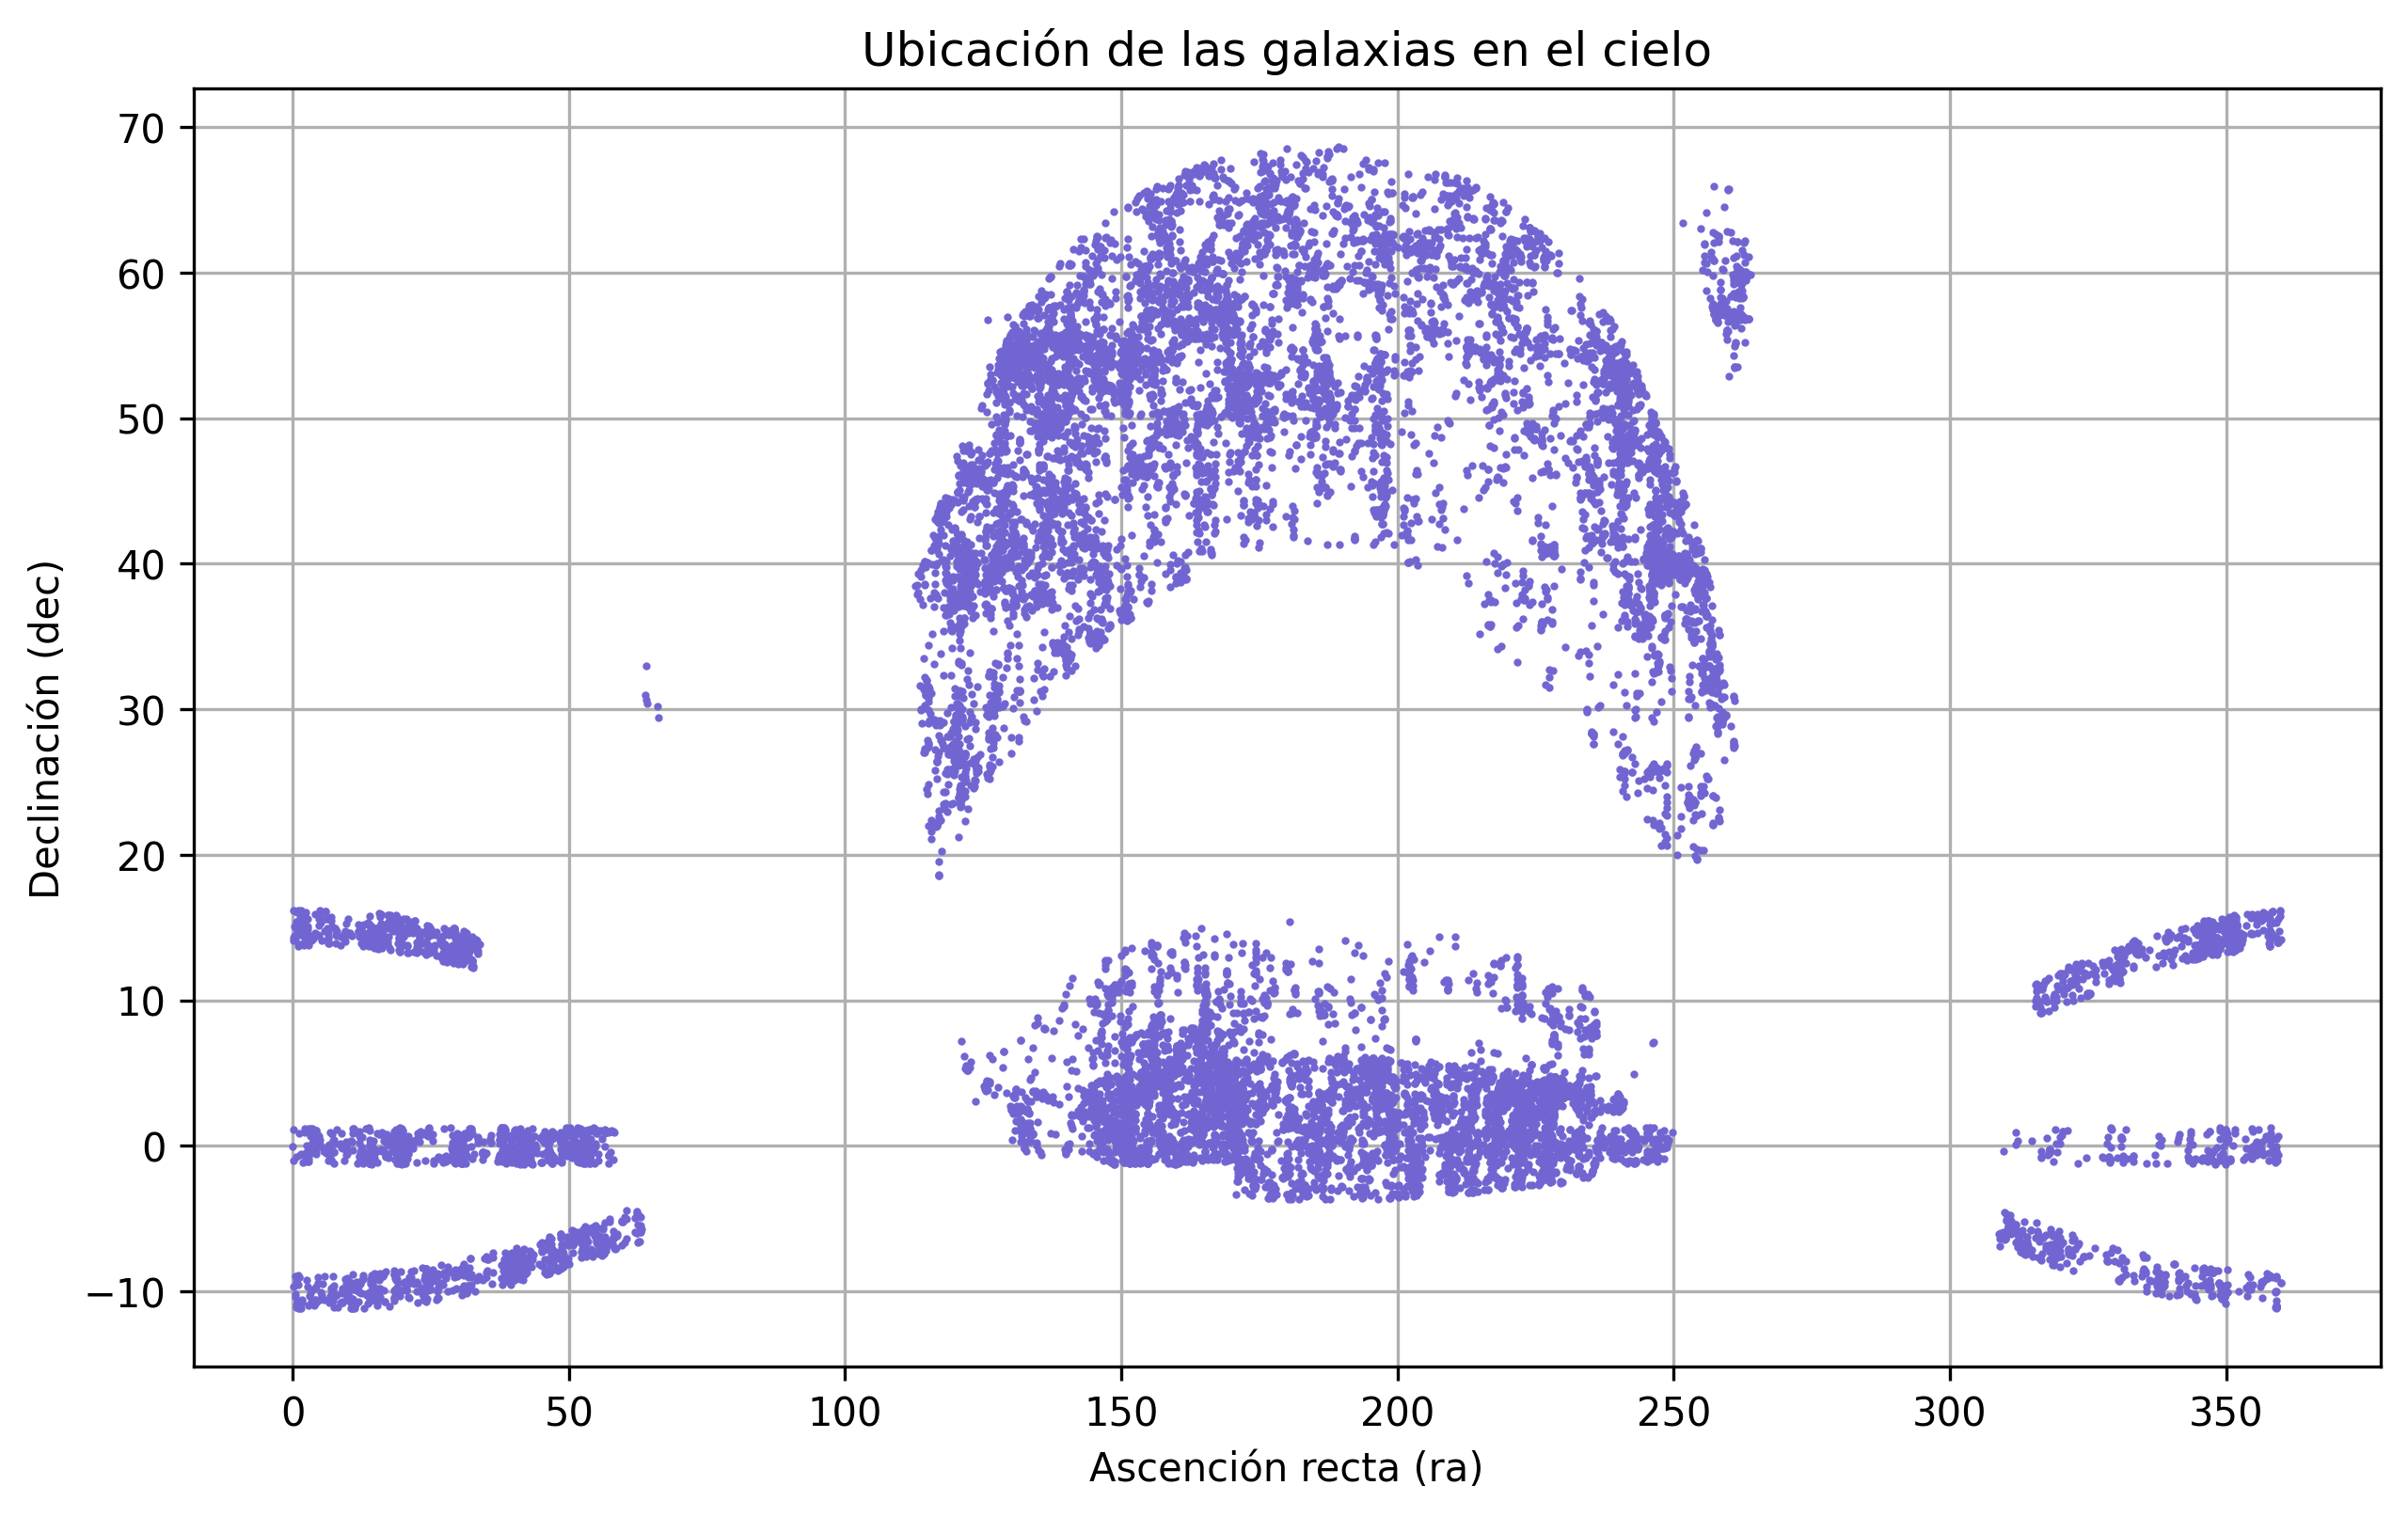
\includegraphics[width=\linewidth]{gal_in_sky.png}
    \caption{Ubicación en el cielo de las galaxias seleccionadas.}
    \label{fig:araña}
\end{figure}

\begin{figure}[ht]
    \centering
    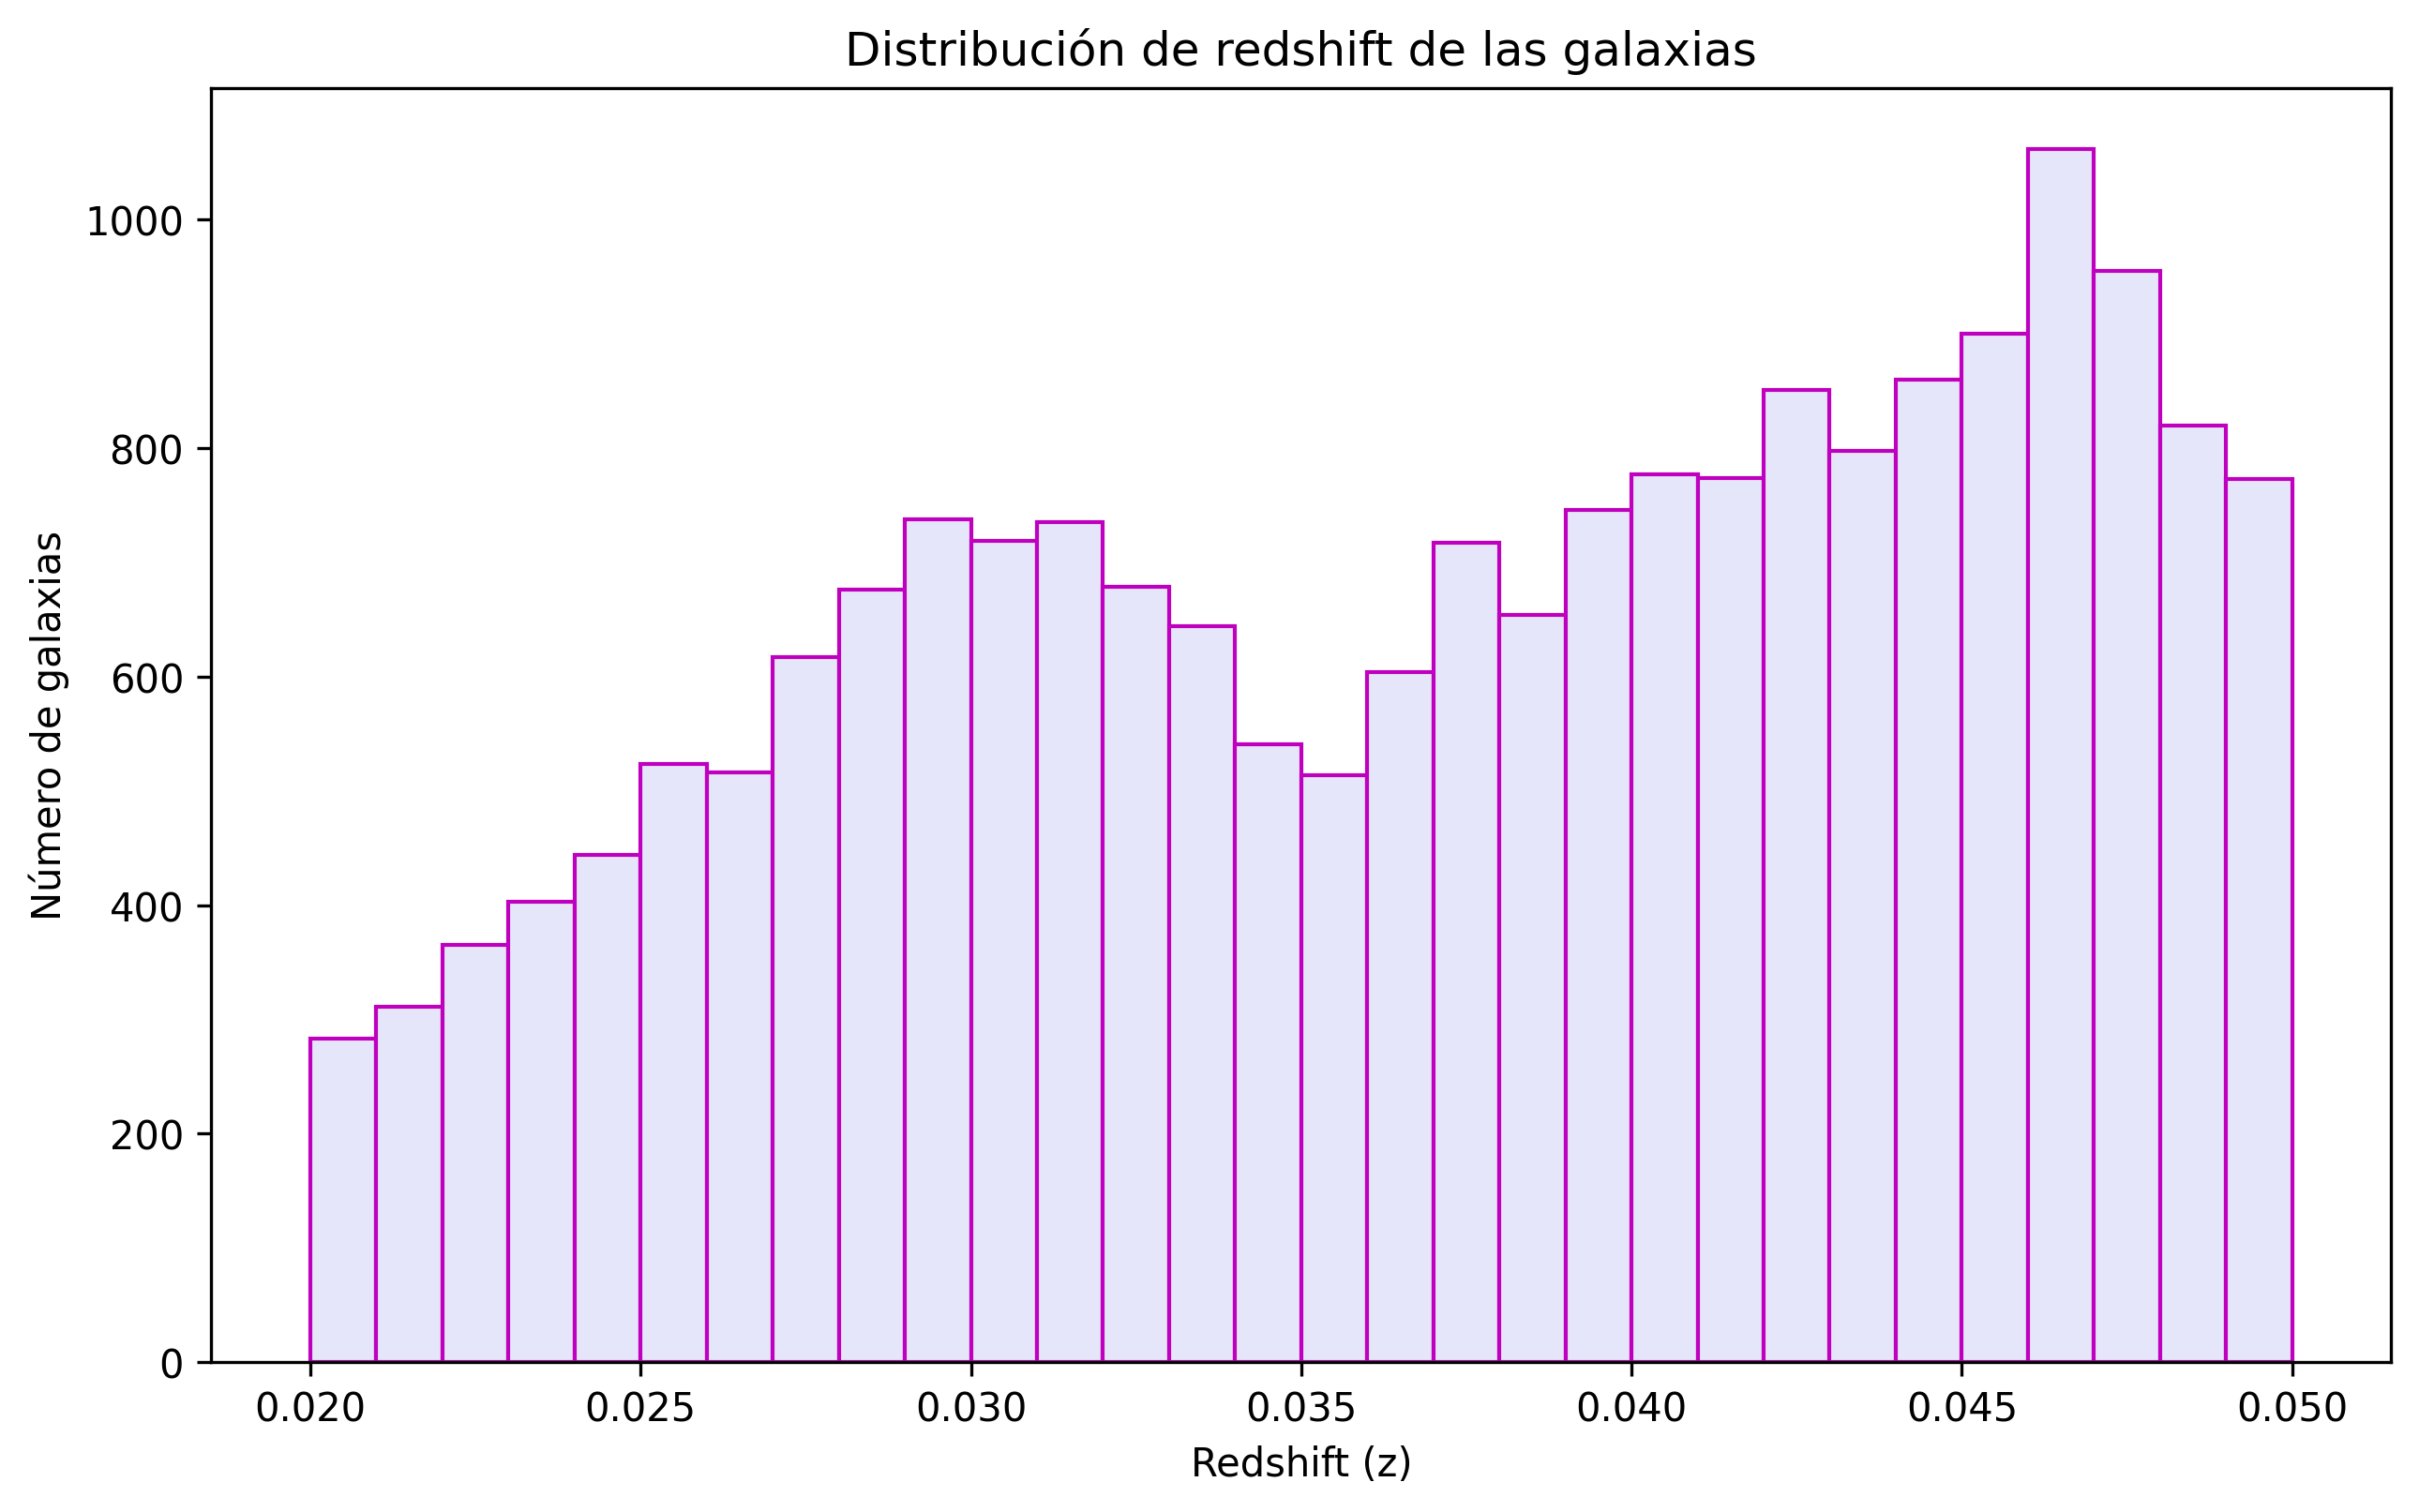
\includegraphics[width=\linewidth]{gal_z.png}
    \caption{Distribución del redshift de las galaxias seleccionadas.}
    \label{fig:hist_z}
\end{figure}

\begin{figure}[ht]
    \centering
    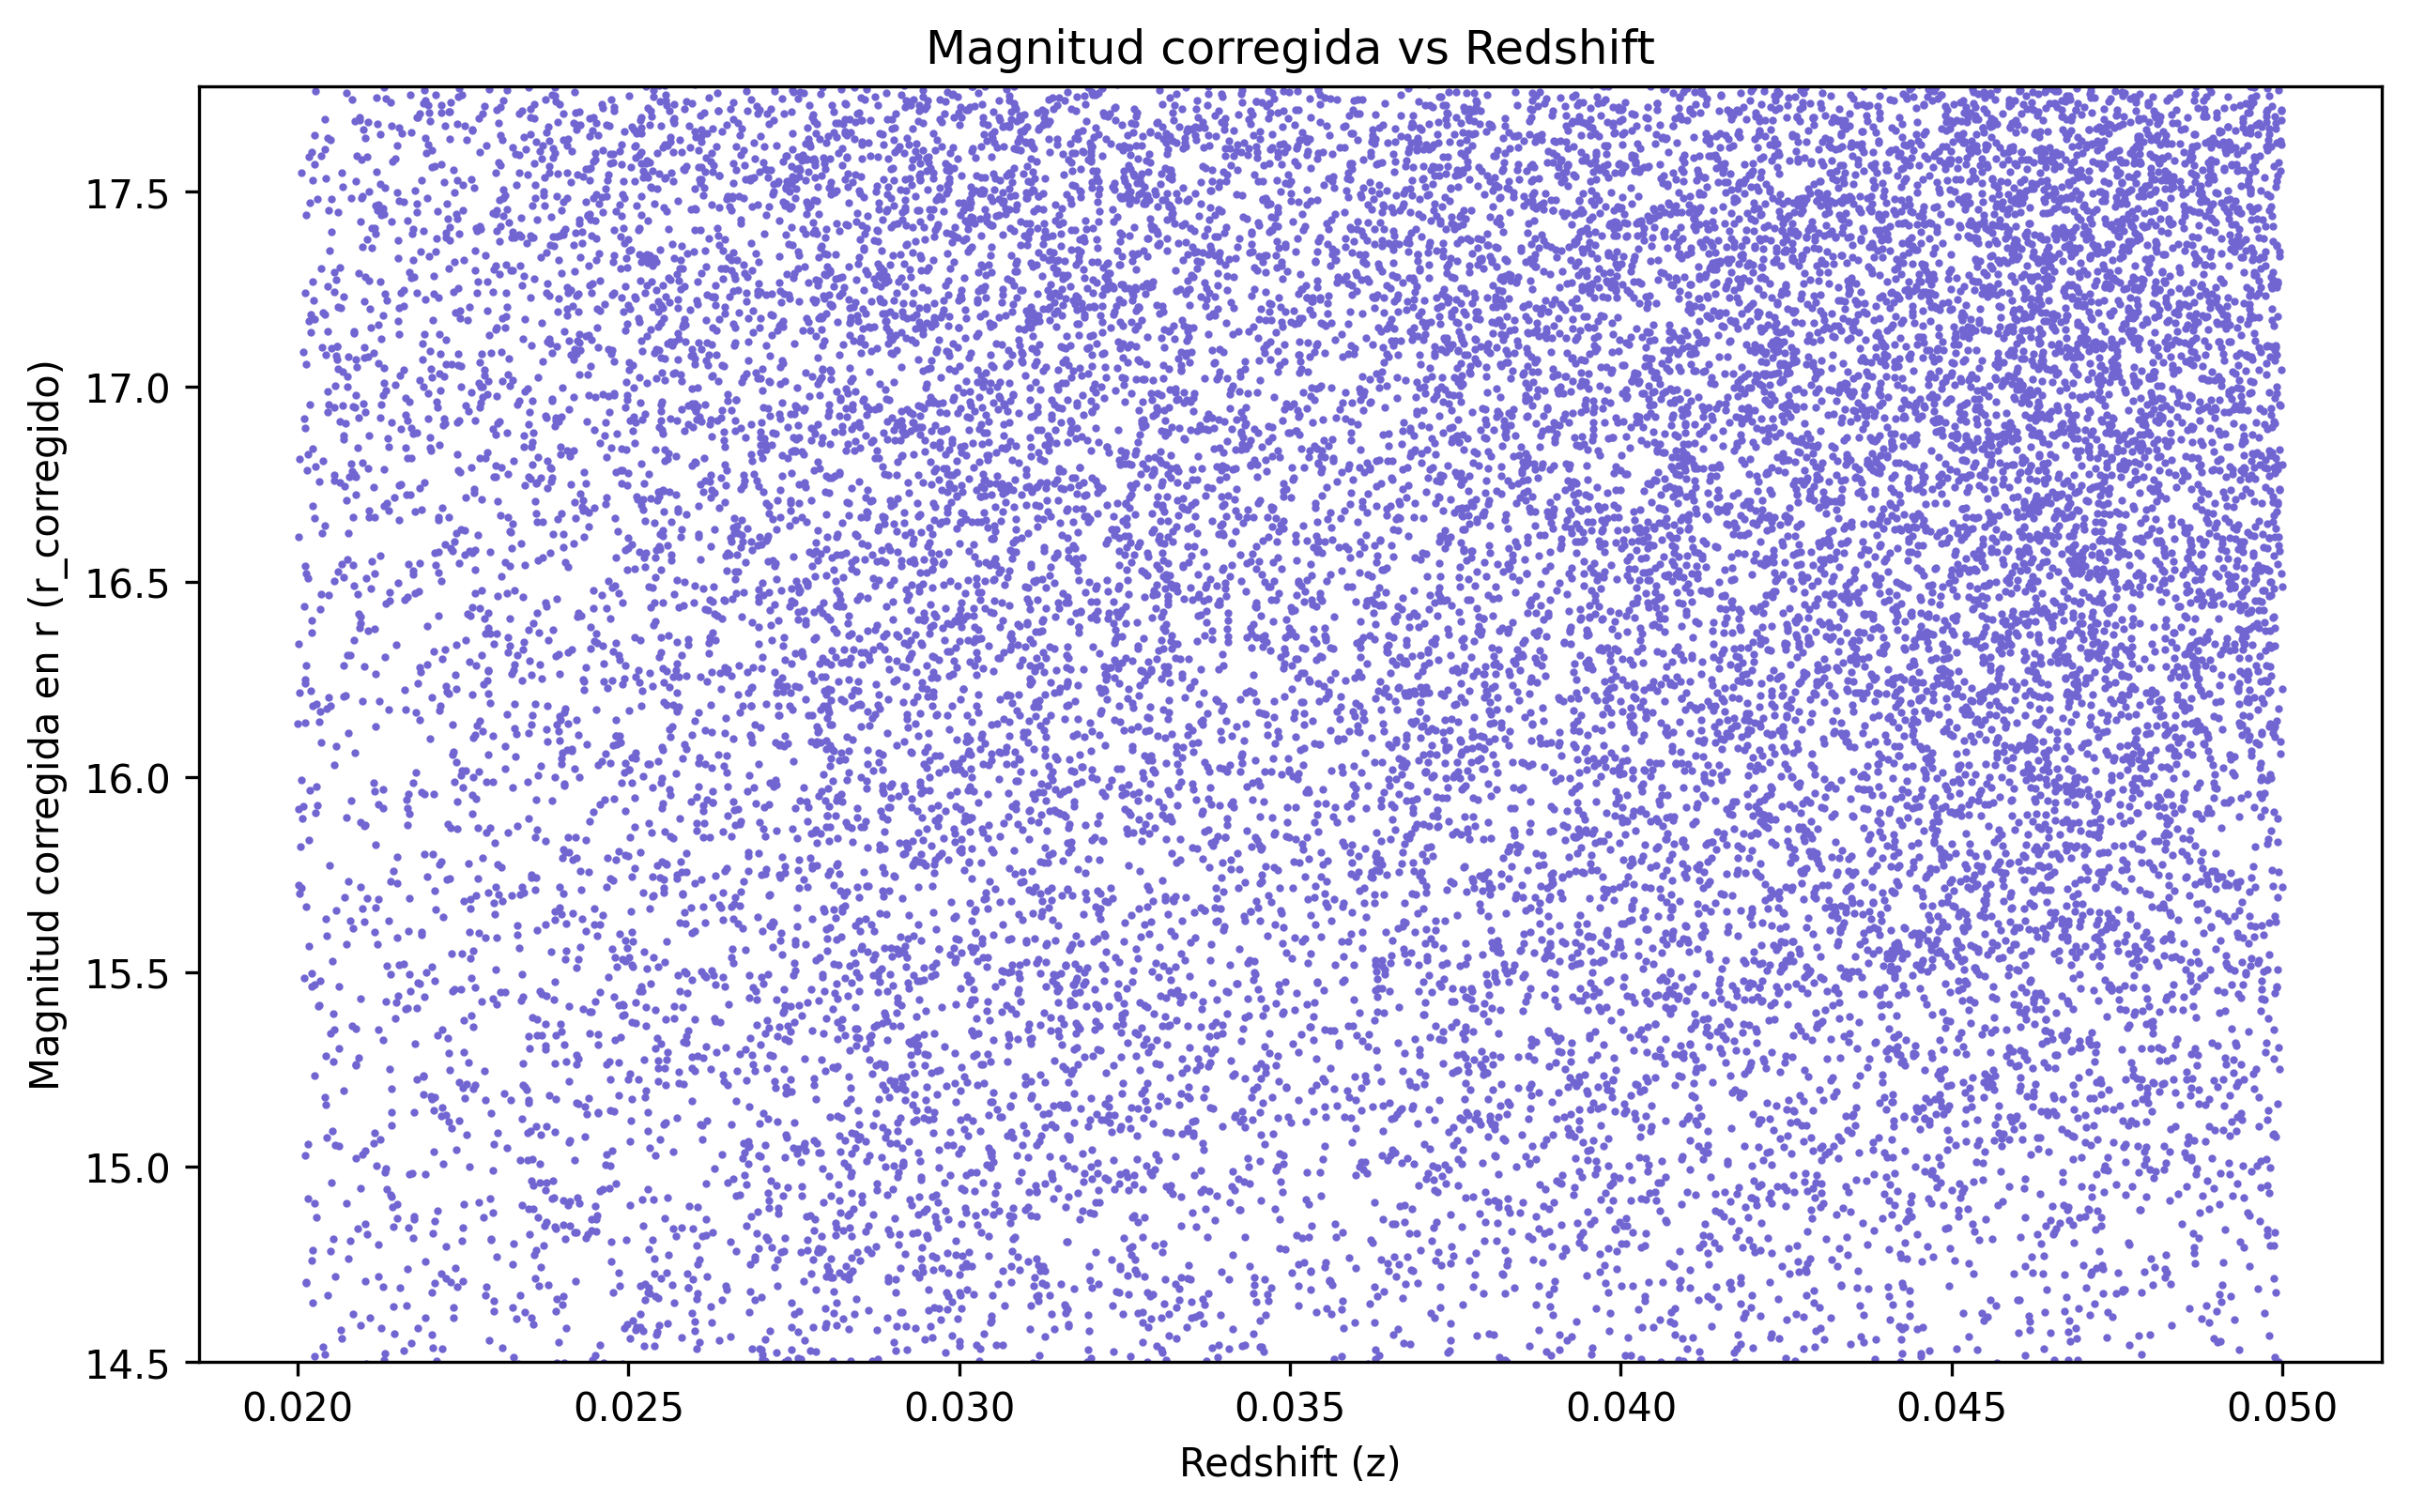
\includegraphics[width=\linewidth]{mag_vs_z.png}
    \caption{Distribución de magnitud aparente vs. redshift.}
    \label{fig:completo_flujo}
\end{figure}

\section{Resultados y discusión}

\subsection{Magnitud absoluta}

Usando $H_0 = 70$ km s$^{-1}$ Mpc$^{-1}$, $\Omega_m = 0.3$, $\Omega_\Lambda = 0.7$, se calcula la distancia luminosa:
\begin{equation}
    d_L = (1 + z)\frac{c}{H_0} \int_0^z \frac{dz'}{\sqrt{\Omega_m(1+z')^3 + \Omega_\Lambda}}
\end{equation}

La magnitud absoluta se calcula como:
\begin{equation}
    M_i = m_i - \text{ext}_i + \text{corr-AB}_i - 5\log_{10}(d_L) - 25
\end{equation}
para $i = (u, g, r, i, z)$.

La Figura \ref{fig:M_r_hist} muestra que la muestra no es completa en volumen, con distribución que varía con el redshift.

\begin{figure}[ht]
    \centering
    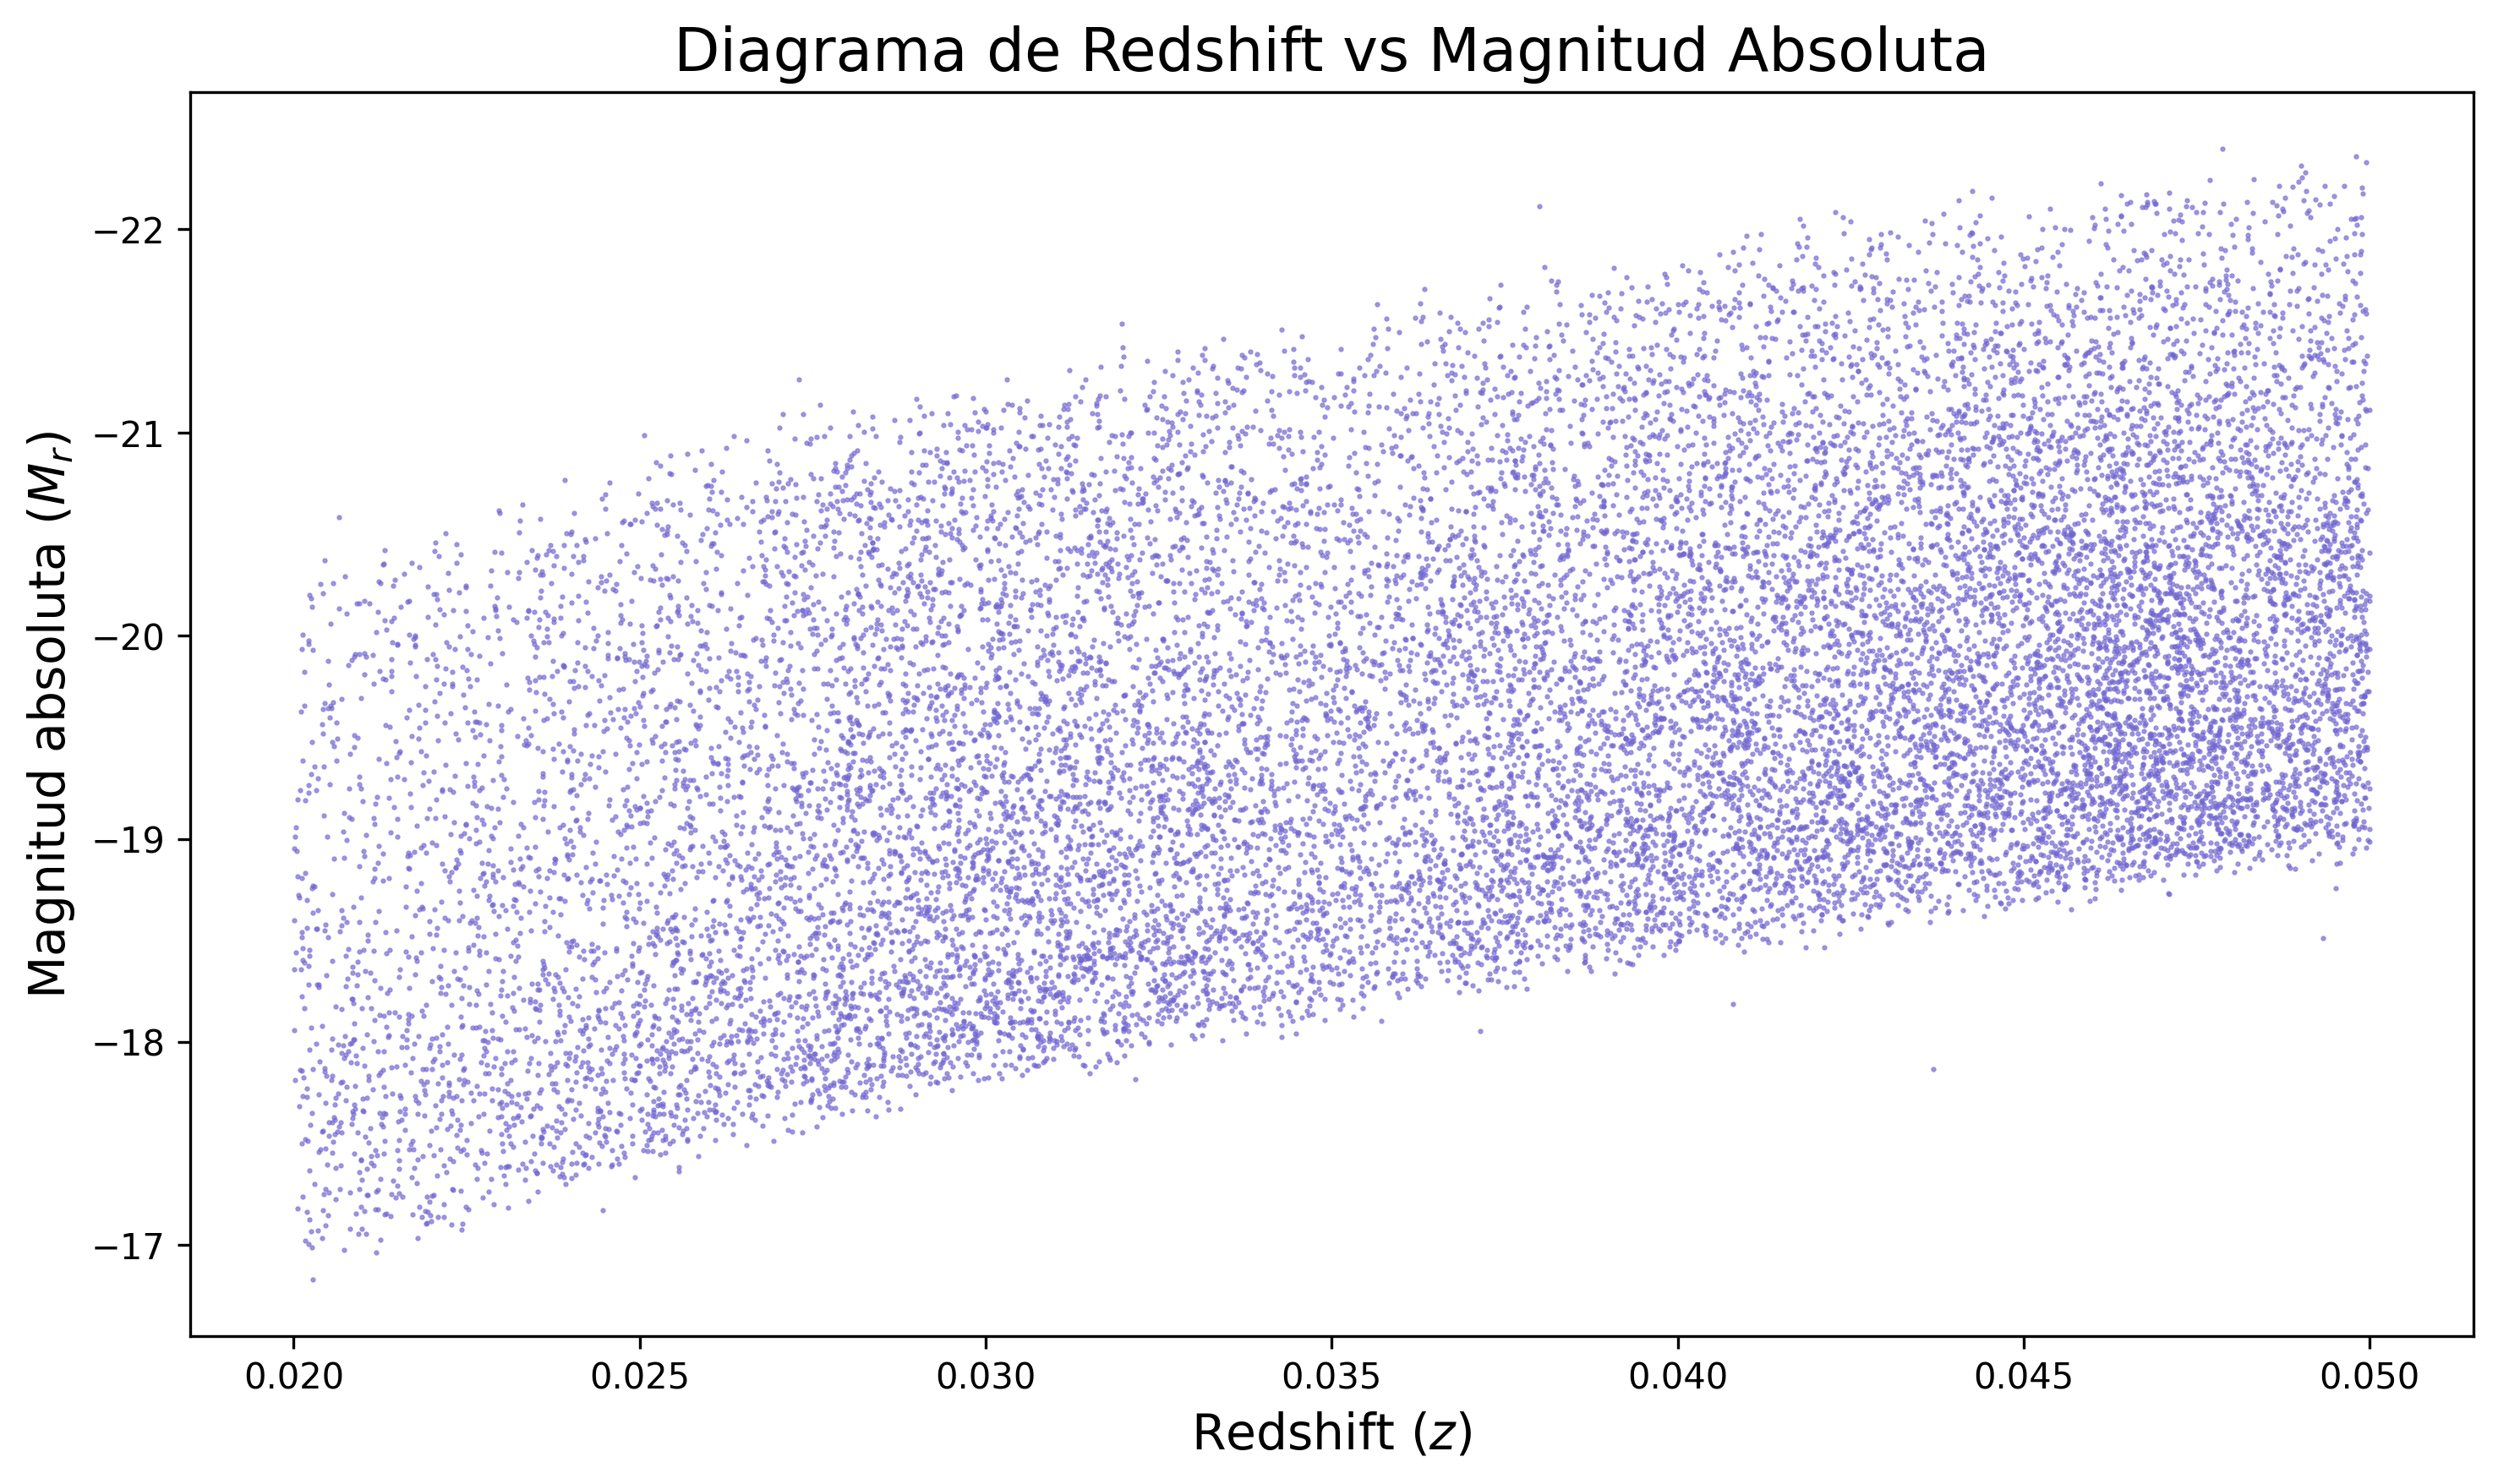
\includegraphics[width=\linewidth]{mabs_vs_z.png}
    \caption{Distribución de magnitud absoluta vs. redshift.}
    \label{fig:M_r_hist}
\end{figure}

\subsection{Índices de color}

Los índices de color muestran rango $(0,4)$ para $u-r$ y $(0,1)$ para $g-r$, con bimodalidad evidente (Figura \ref{fig:colores}) \citep{2004ApJ...600..681B}.

El límite $u-r \sim 2.10$ separa galaxias rojas y azules (Figura \ref{fig:red_blue}).

\begin{figure}[ht]
    \centering
    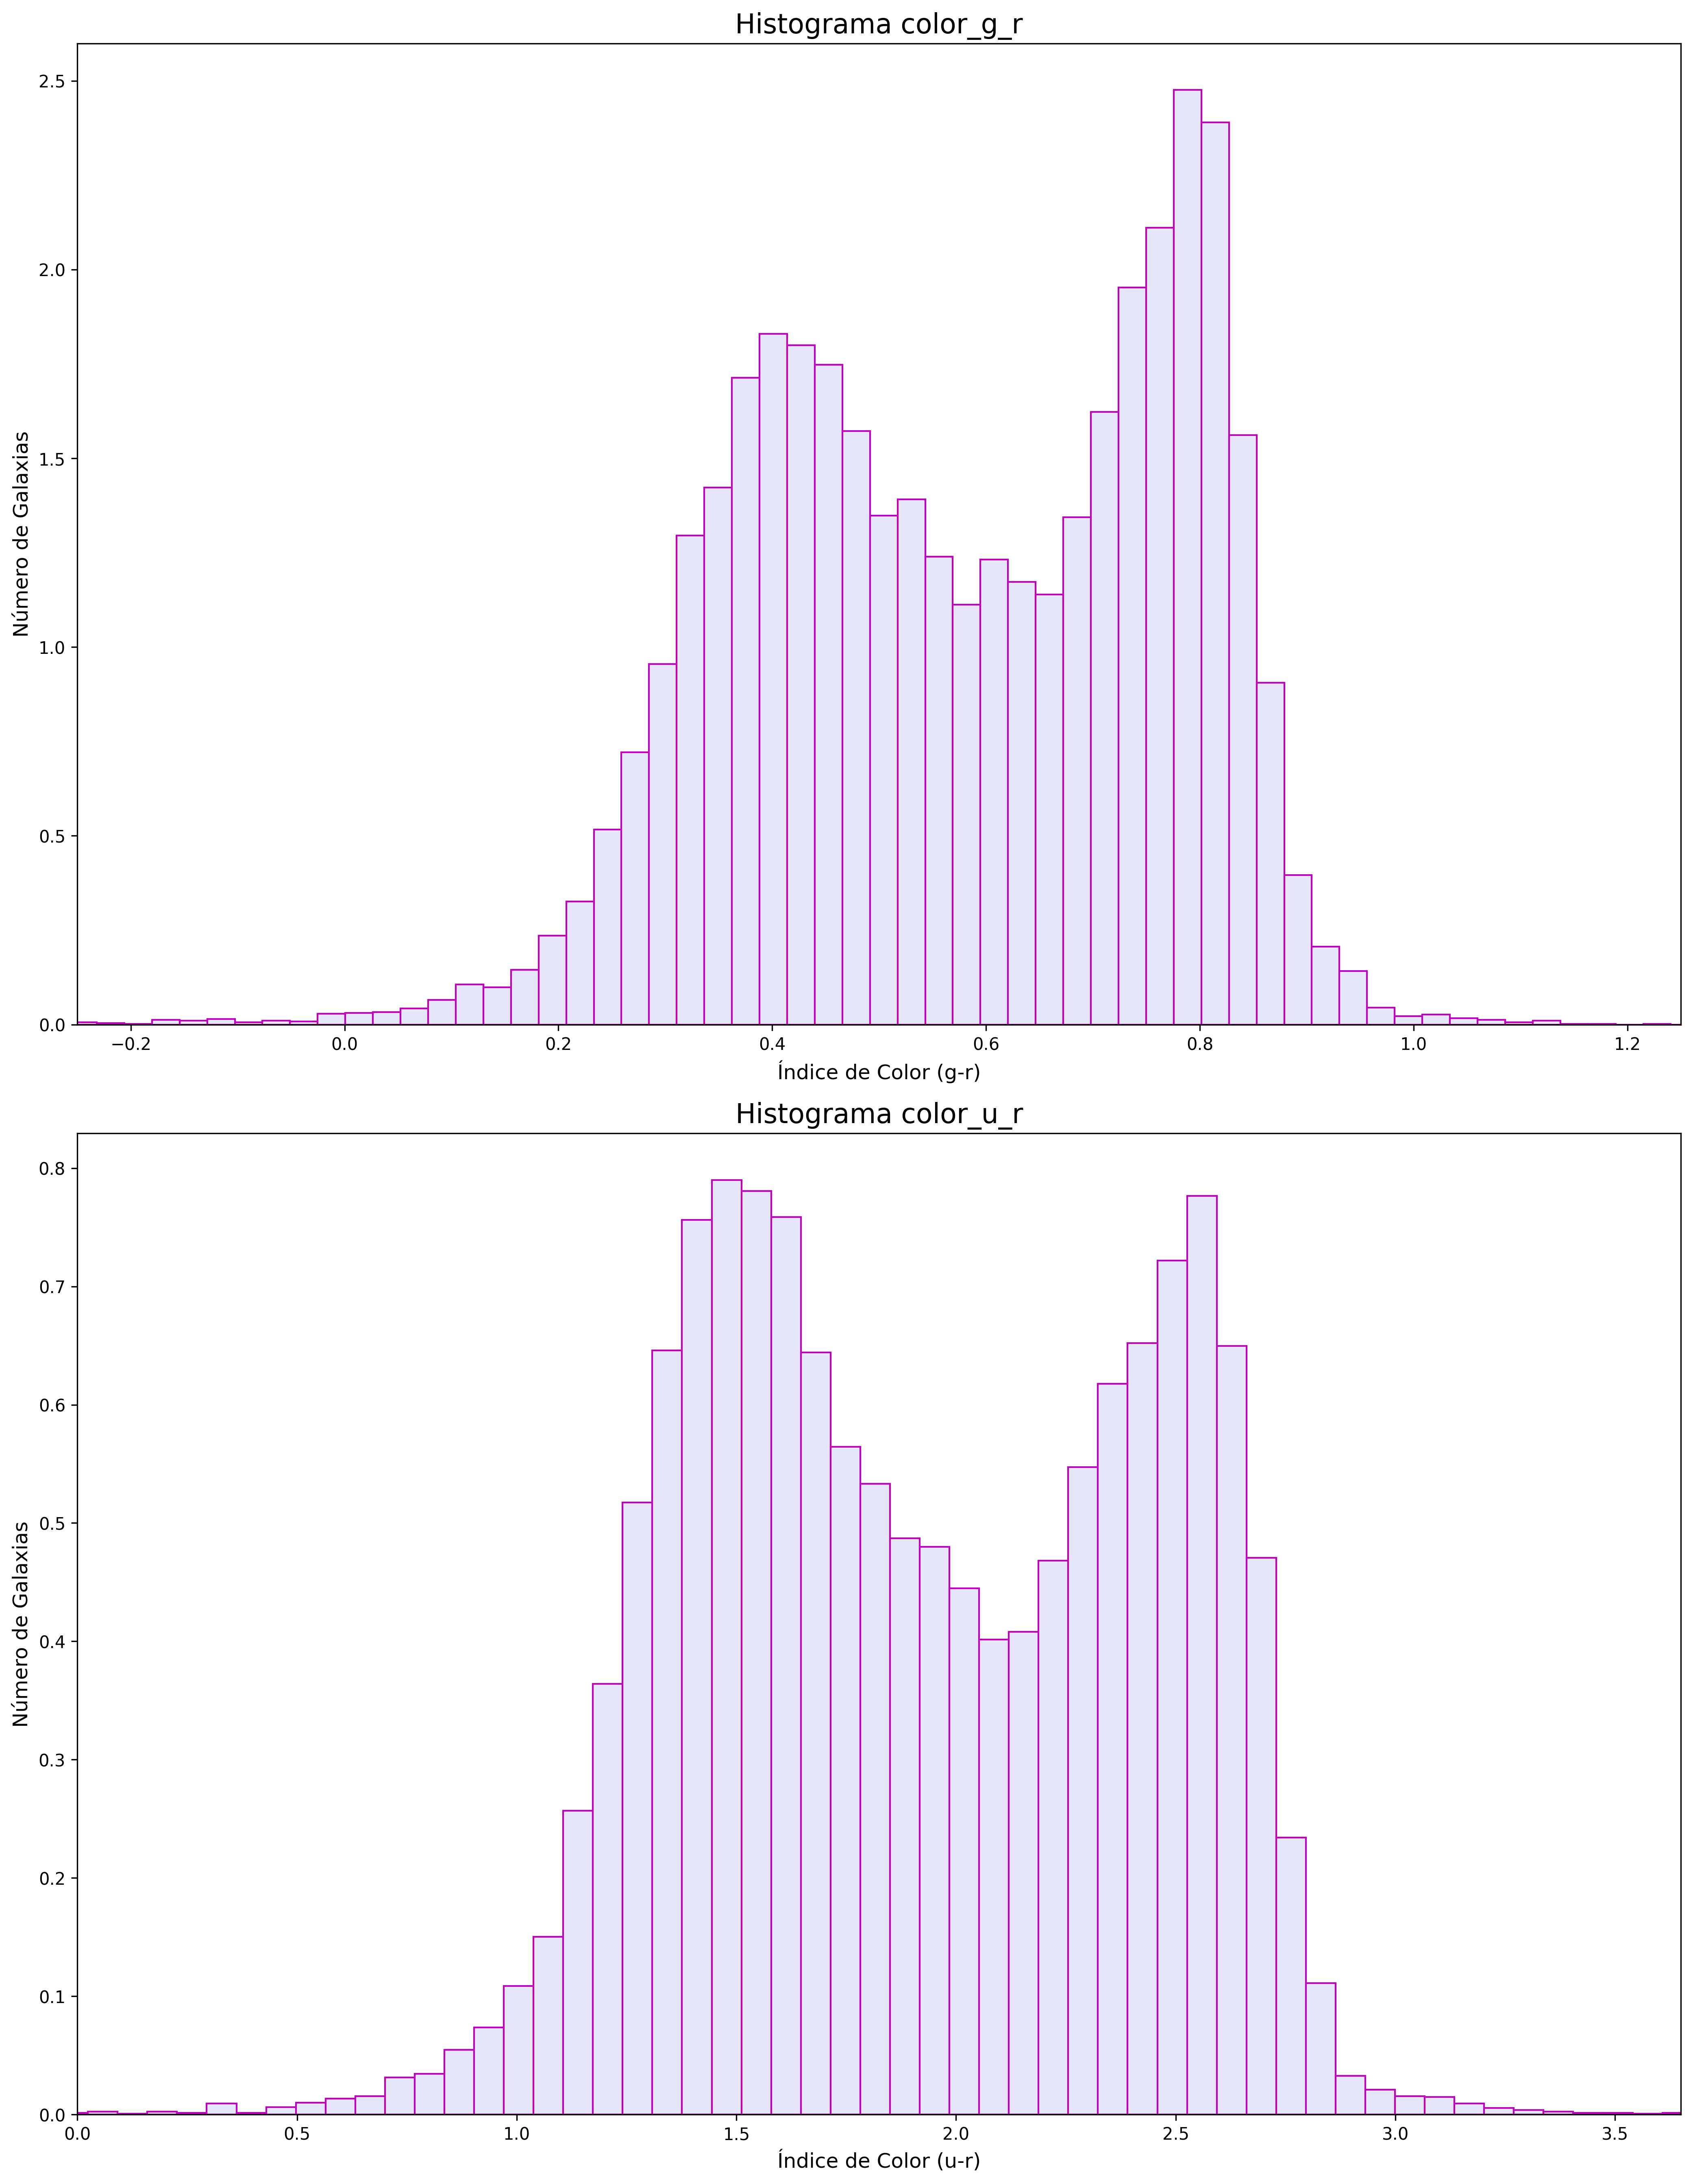
\includegraphics[width=\linewidth]{colores.png}
    \caption{Histograma de los índices de color de las galaxias seleccionadas.}
    \label{fig:colores}
\end{figure}

\begin{figure}[ht]
    \centering
    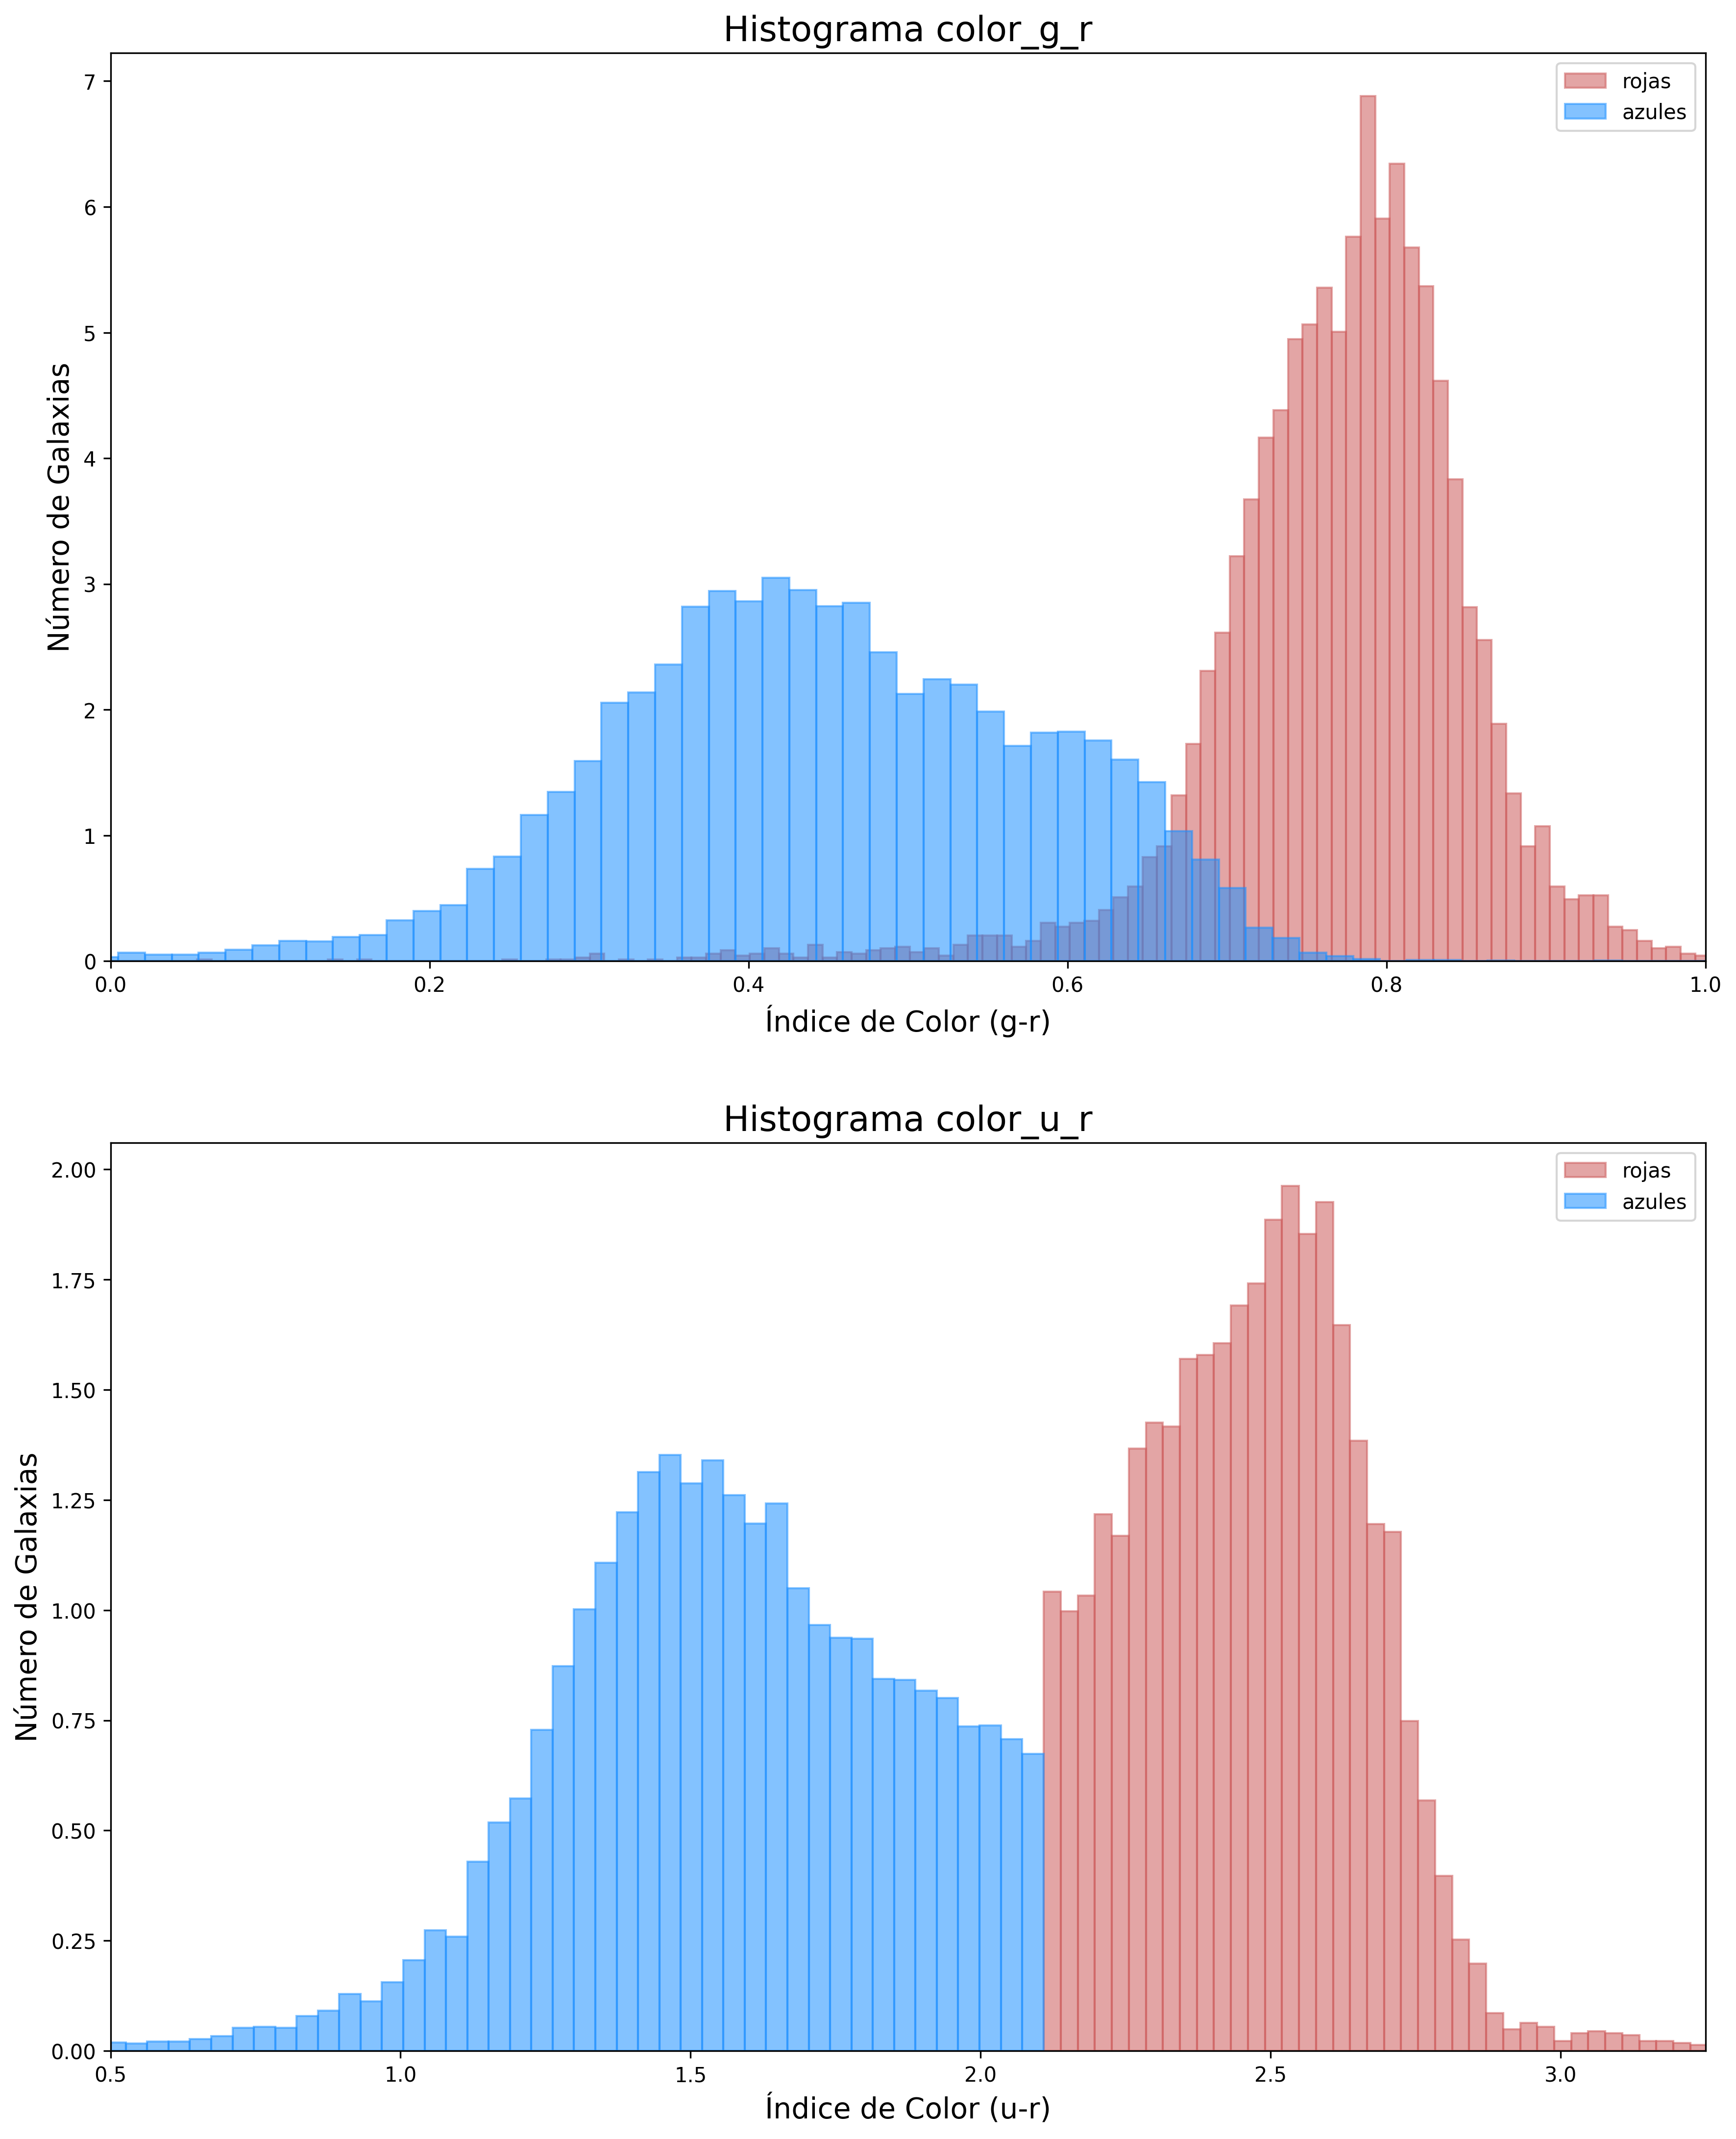
\includegraphics[width=\linewidth]{rojas_y_azules.png}
    \caption{Distribución de galaxias rojas y azules según índice $u-r$.}
    \label{fig:red_blue}
\end{figure}

\subsection{Parámetros de concentración y fracDeV}

La concentración $C$ muestra pico alrededor de 2.5 (Figura \ref{fig:hist_c}), usado para separar galaxias tempranas ($C > 2.5$) y tardías ($C \leq 2.5$).

El parámetro fracDeV muestra sobredensidades en 0 (discos) y 1 (bulbos) (Figura \ref{fig:hist_fracdev}).

La Figura \ref{fig:fracdev_vs_c} muestra correlación débil entre fracDeV y concentración, con bulbos tendiendo a mayor $C$.

\begin{figure}[ht]
    \centering
    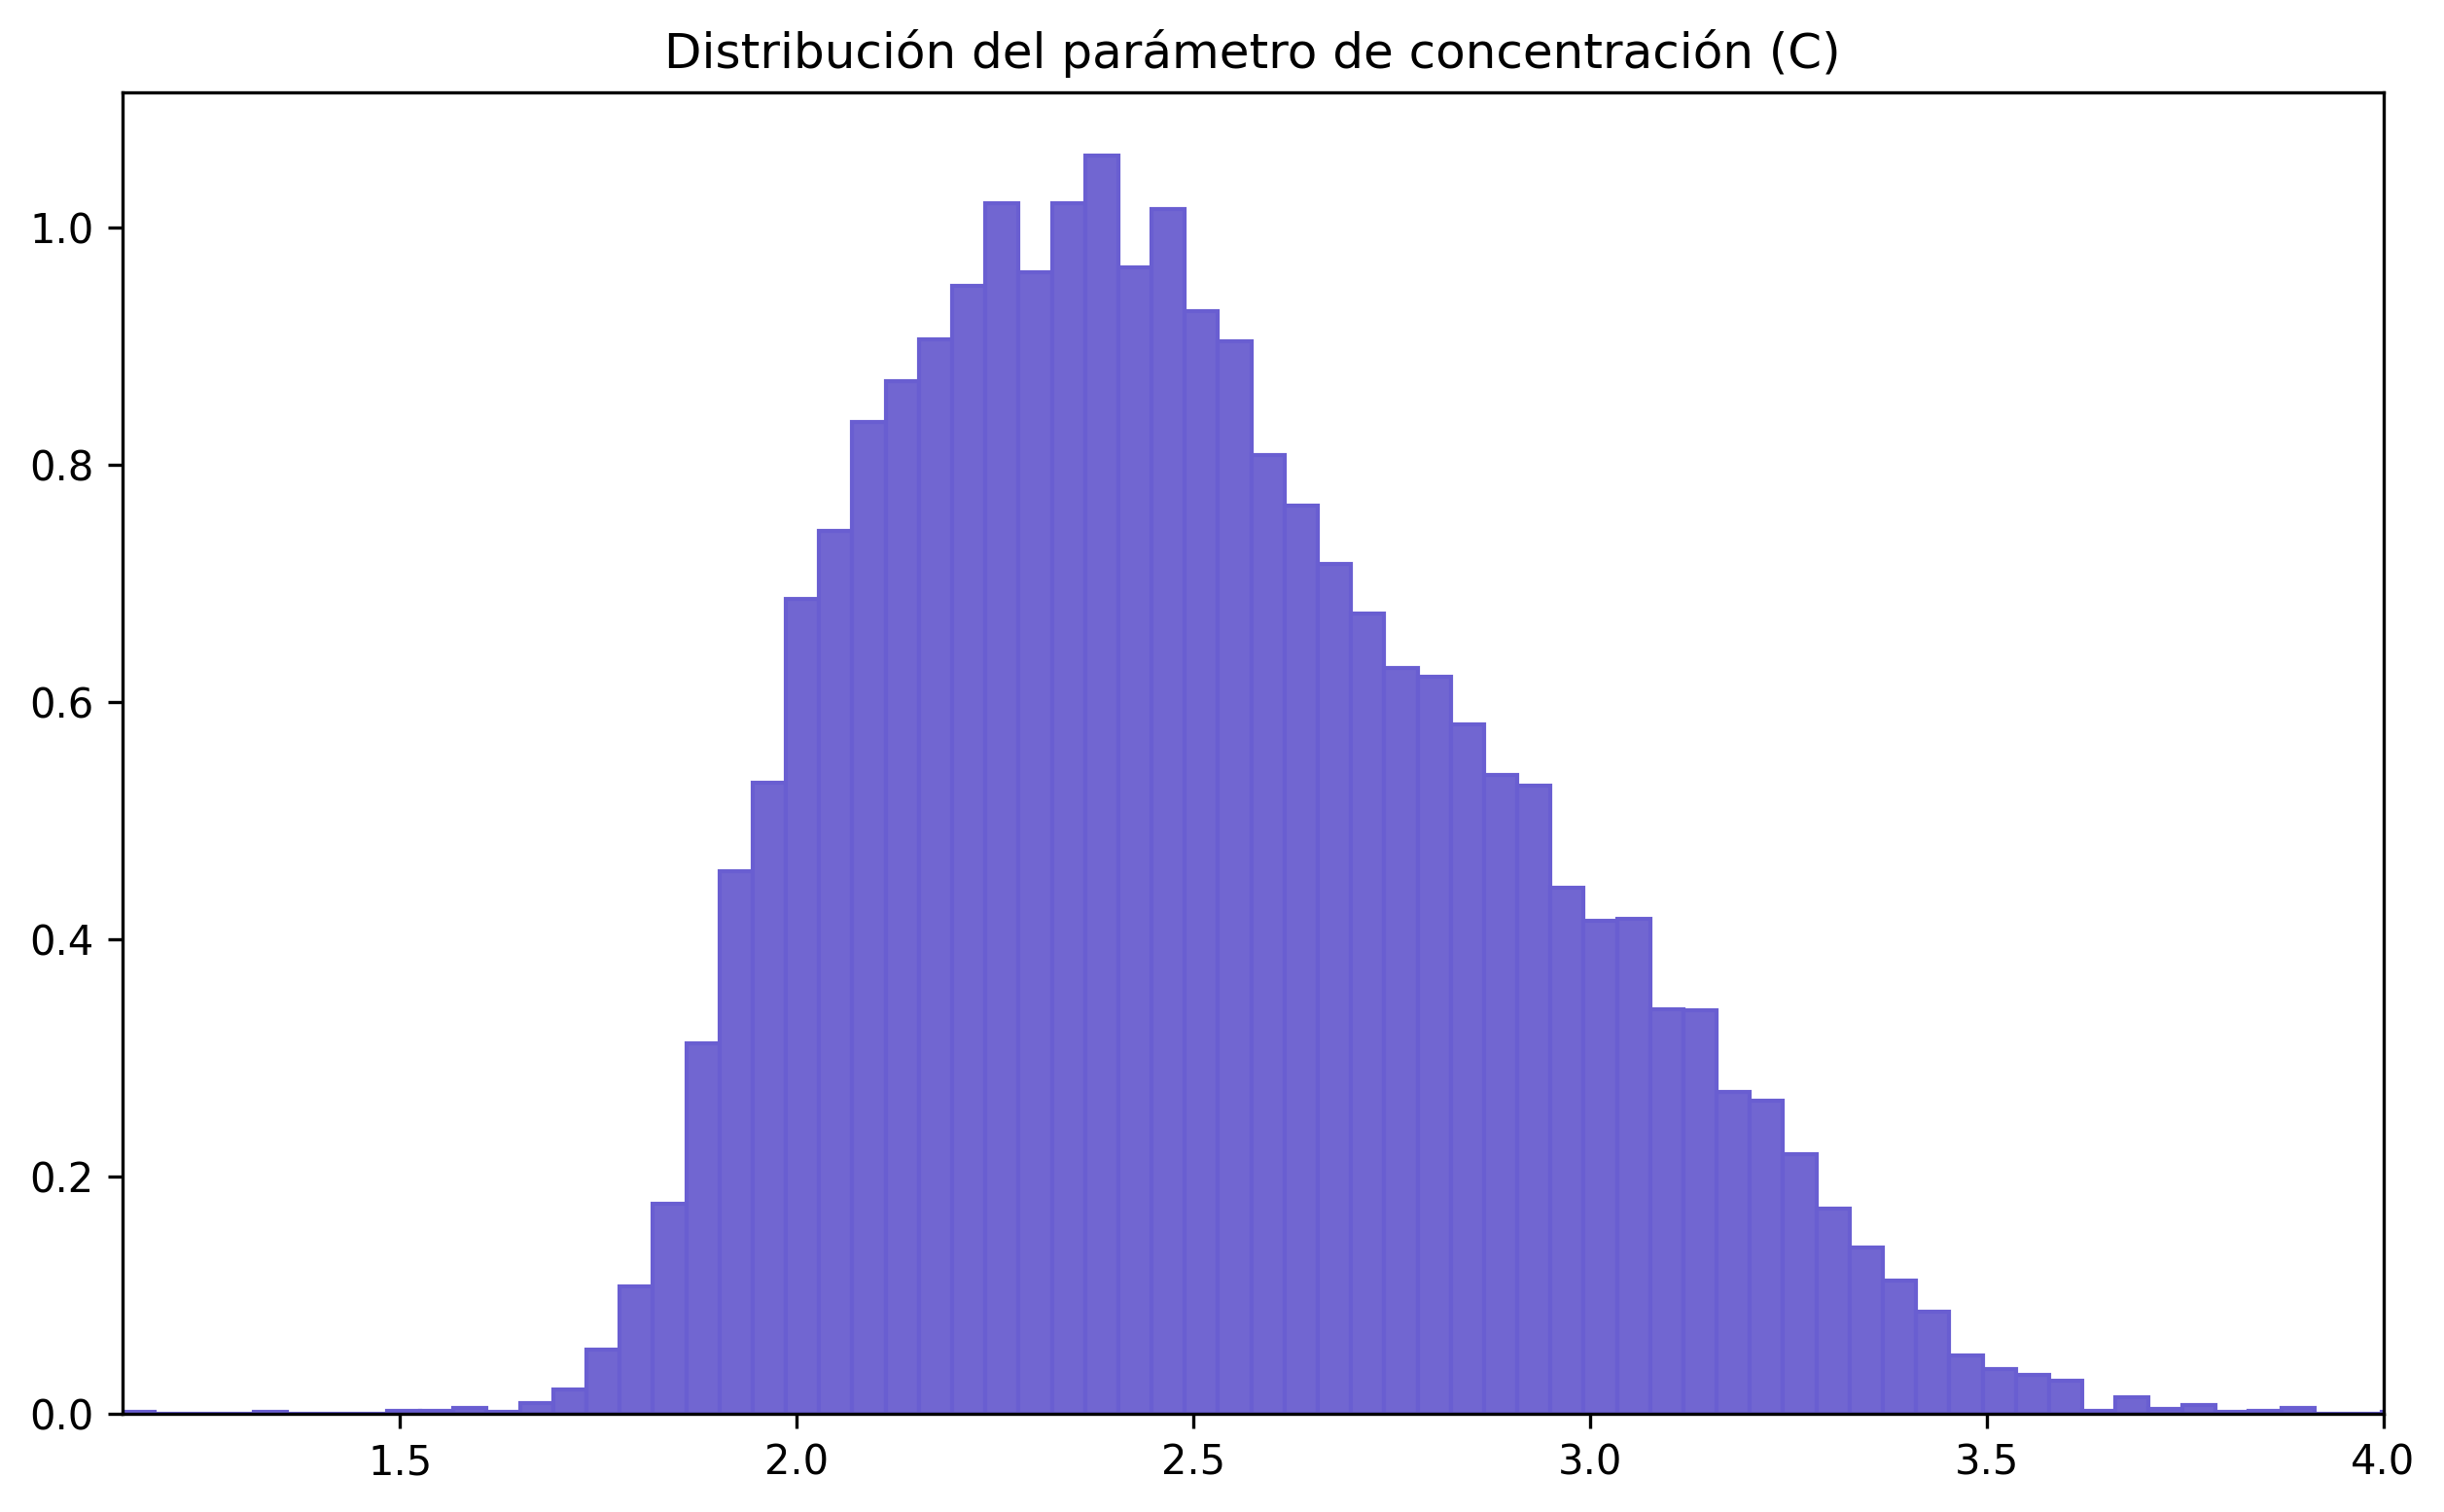
\includegraphics[width=\linewidth]{hist_c.png}
    \caption{Histograma del parámetro de concentración $r_{50}/r_{90}$.}
    \label{fig:hist_c}
\end{figure}

\begin{figure}[ht]
    \centering
    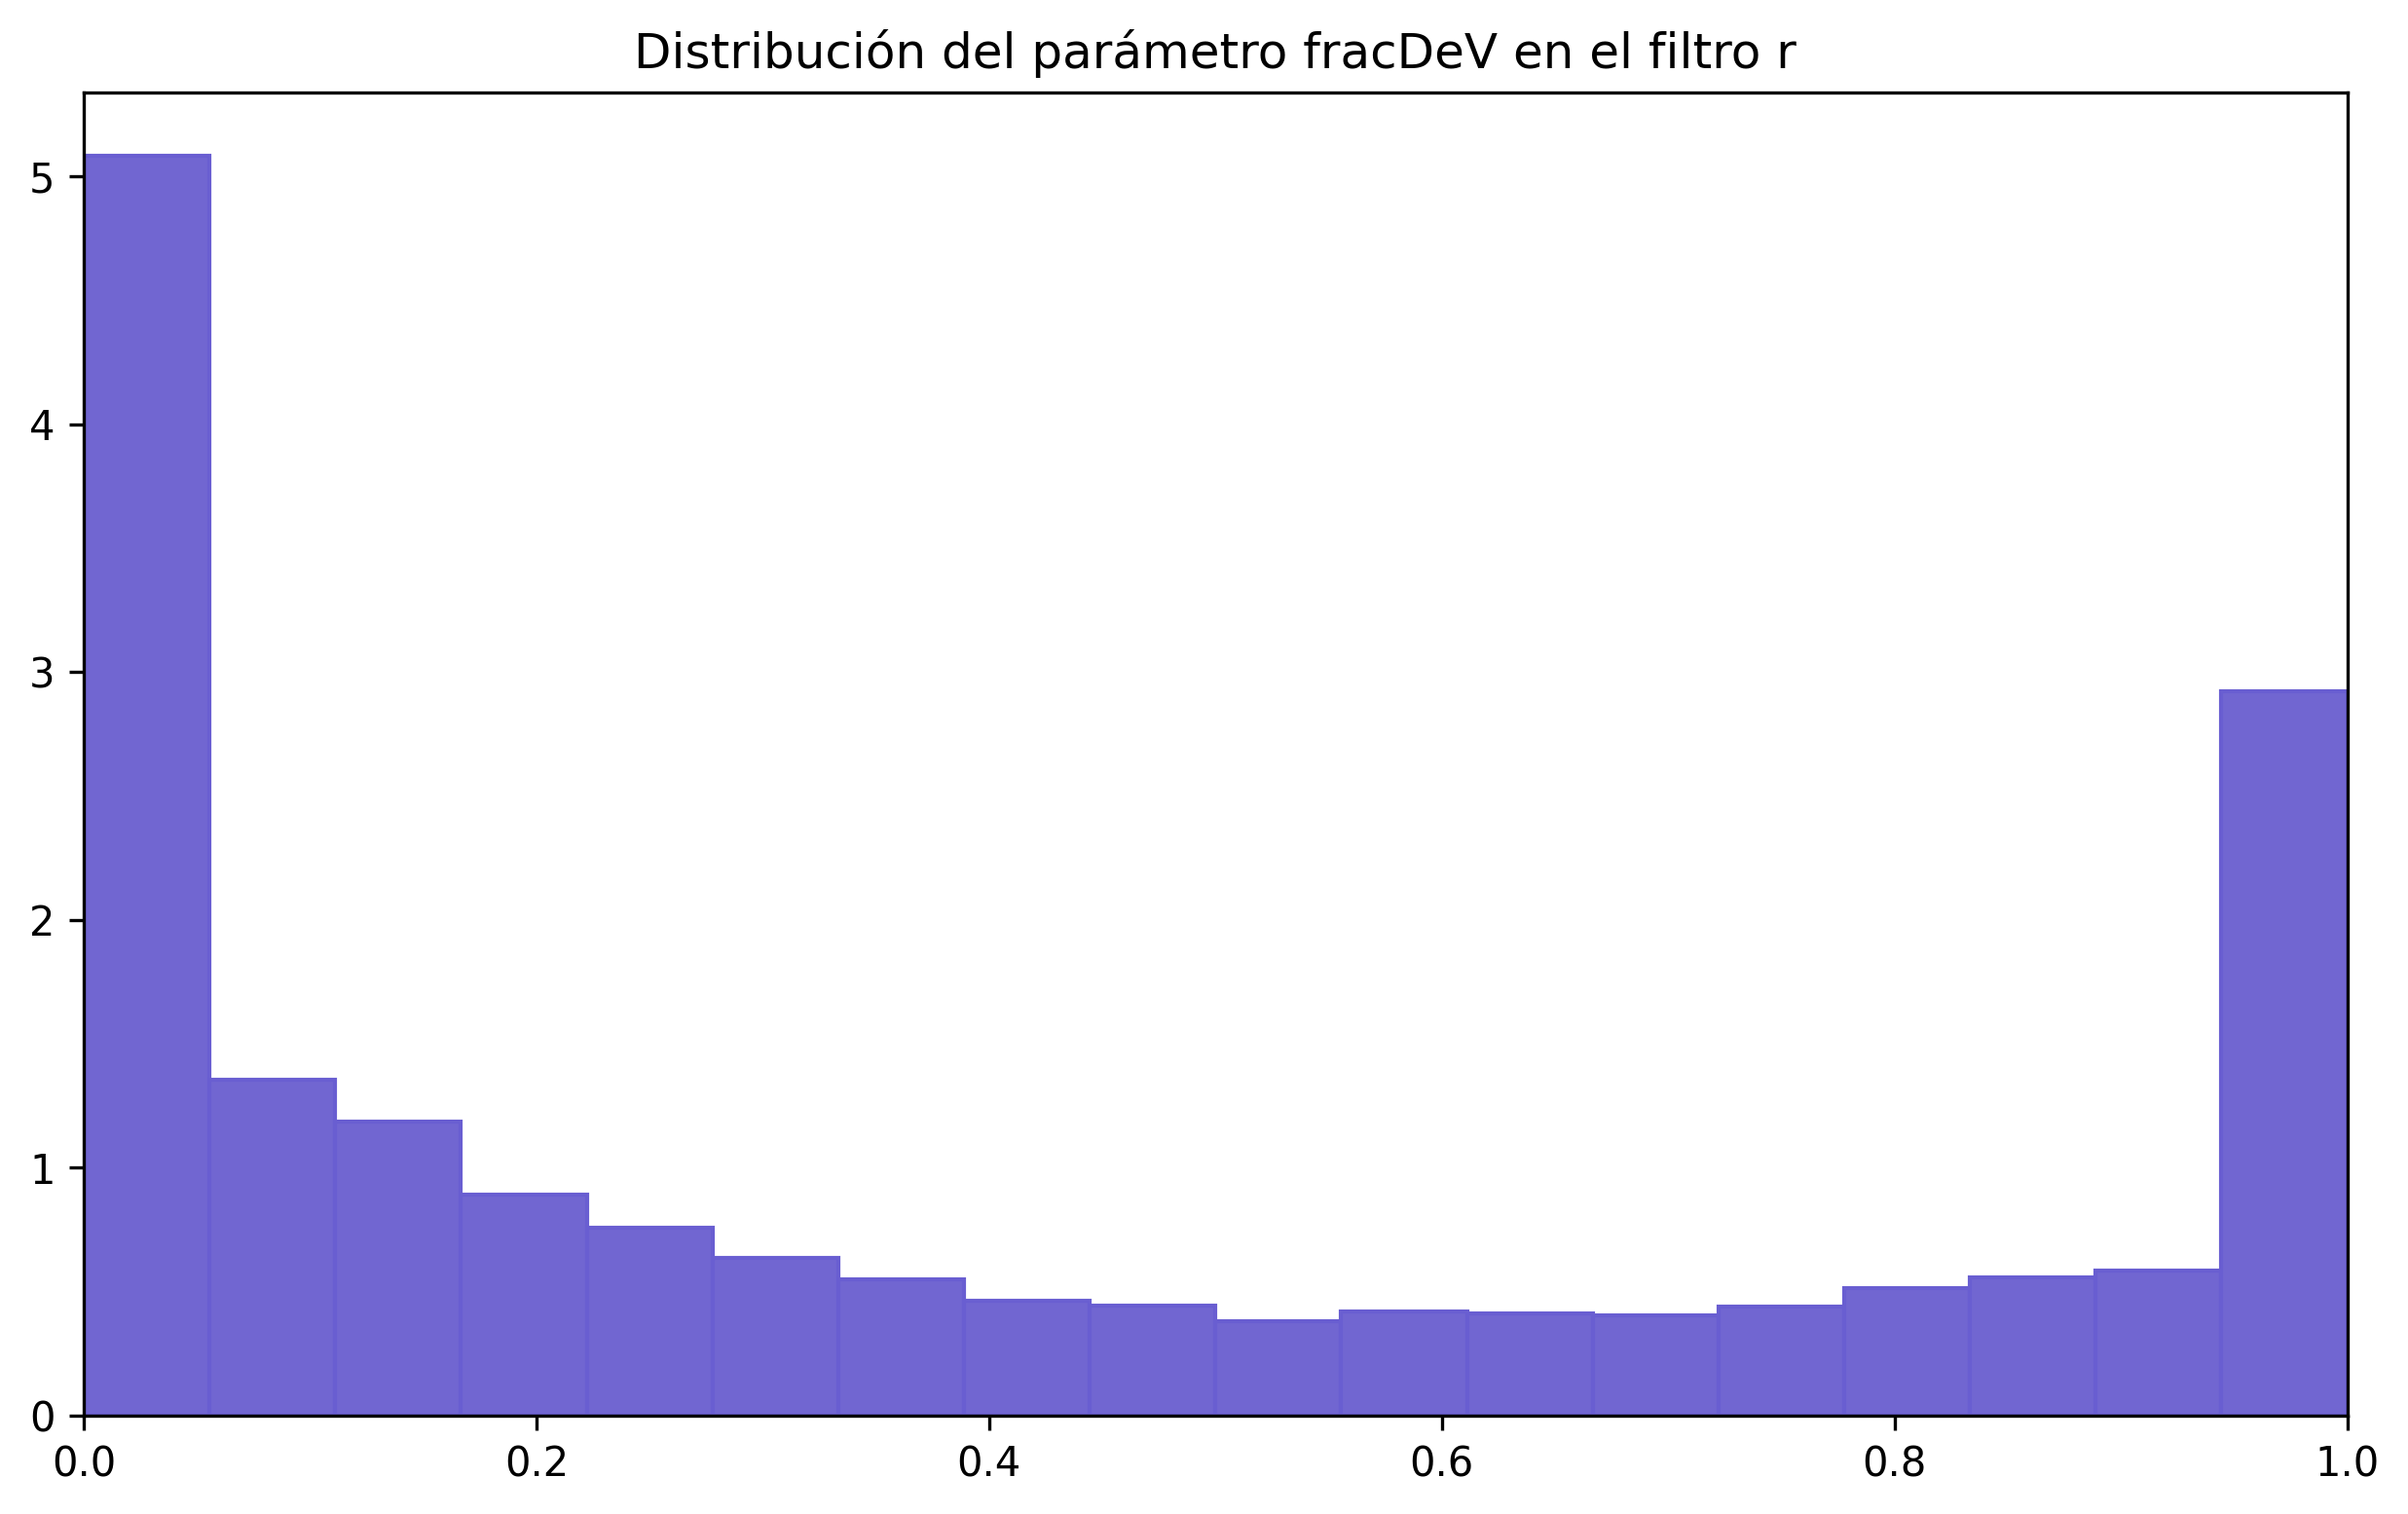
\includegraphics[width=\linewidth]{hist_fracdev.png}
    \caption{Histograma del parámetro fracDeV.}
    \label{fig:hist_fracdev}
\end{figure}

\begin{figure}[ht]
    \centering
    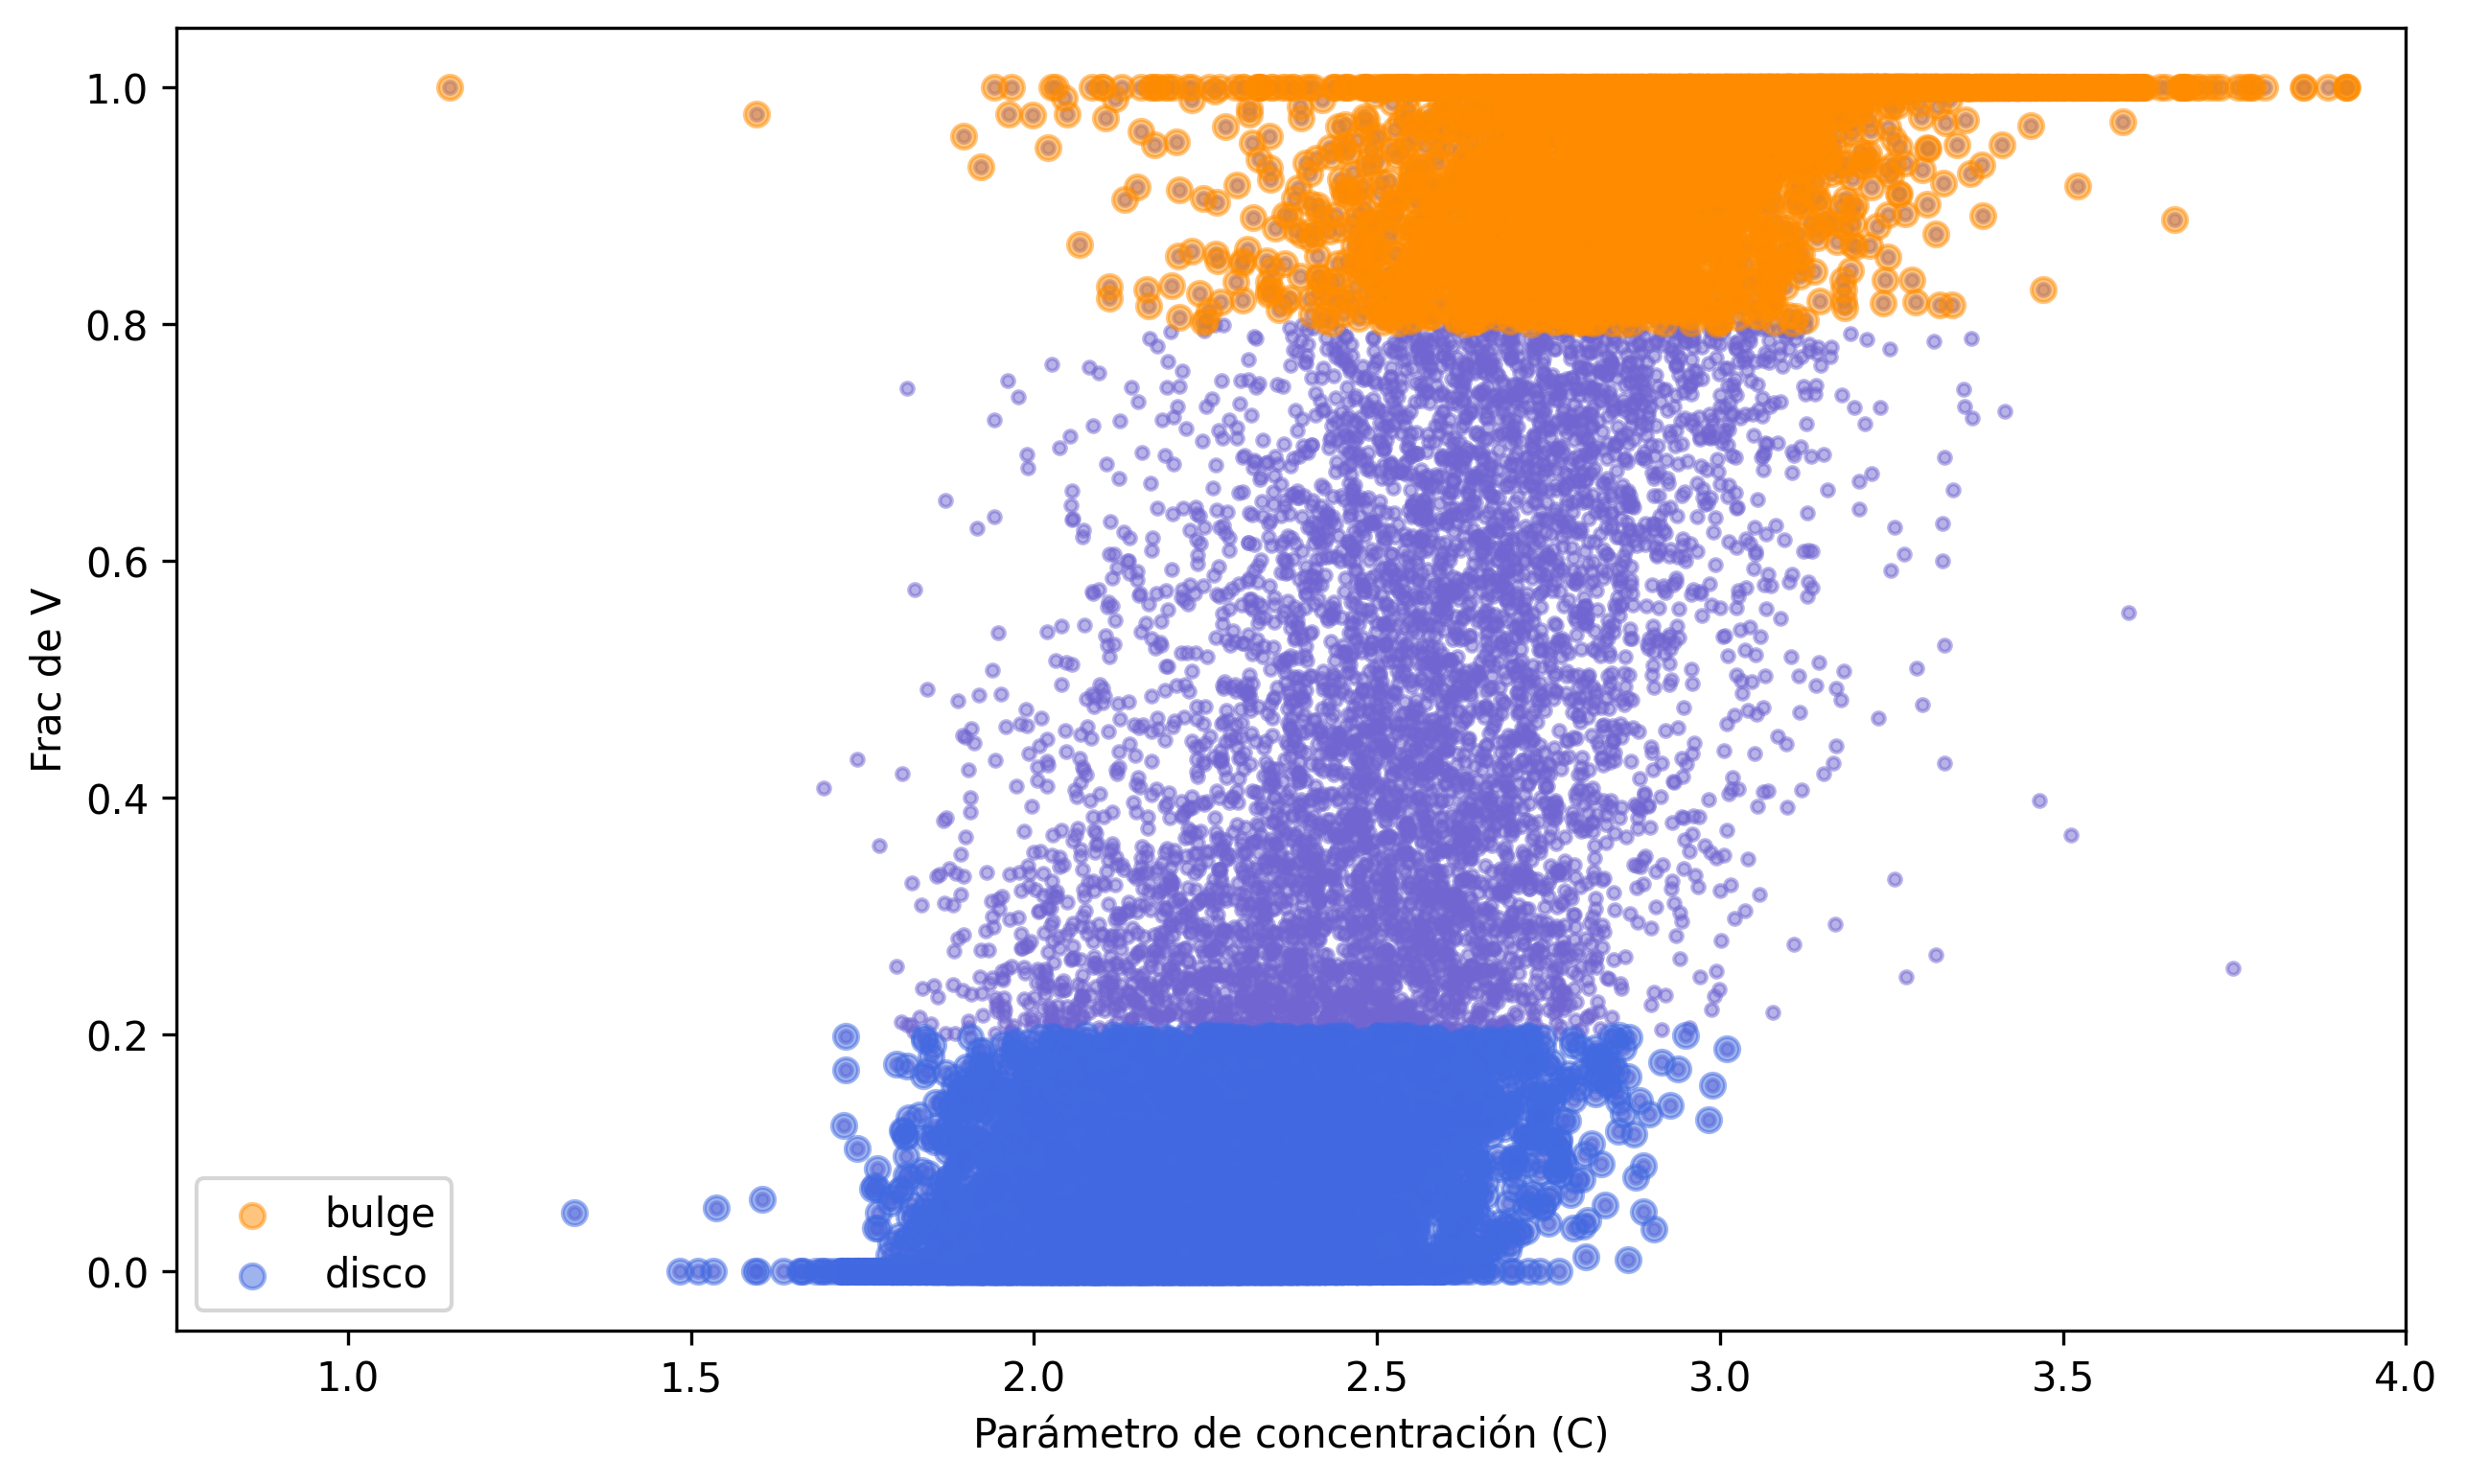
\includegraphics[width=\linewidth]{fracdev_vs_c.png}
    \caption{Parámetro de concentración vs. parámetro fracDeV.}
    \label{fig:fracdev_vs_c}
\end{figure}

\subsection{Relación tamaño-luminosidad}

Las Figuras \ref{fig:mabs_vs_r50}--\ref{fig:mabs_vs_r50_earlyylate} muestran relaciones lineales en escala logarítmica. Galaxias azules se ubican sobre galaxias rojas, siendo más brillantes con mayores radios.

\begin{figure}[ht]
    \centering
    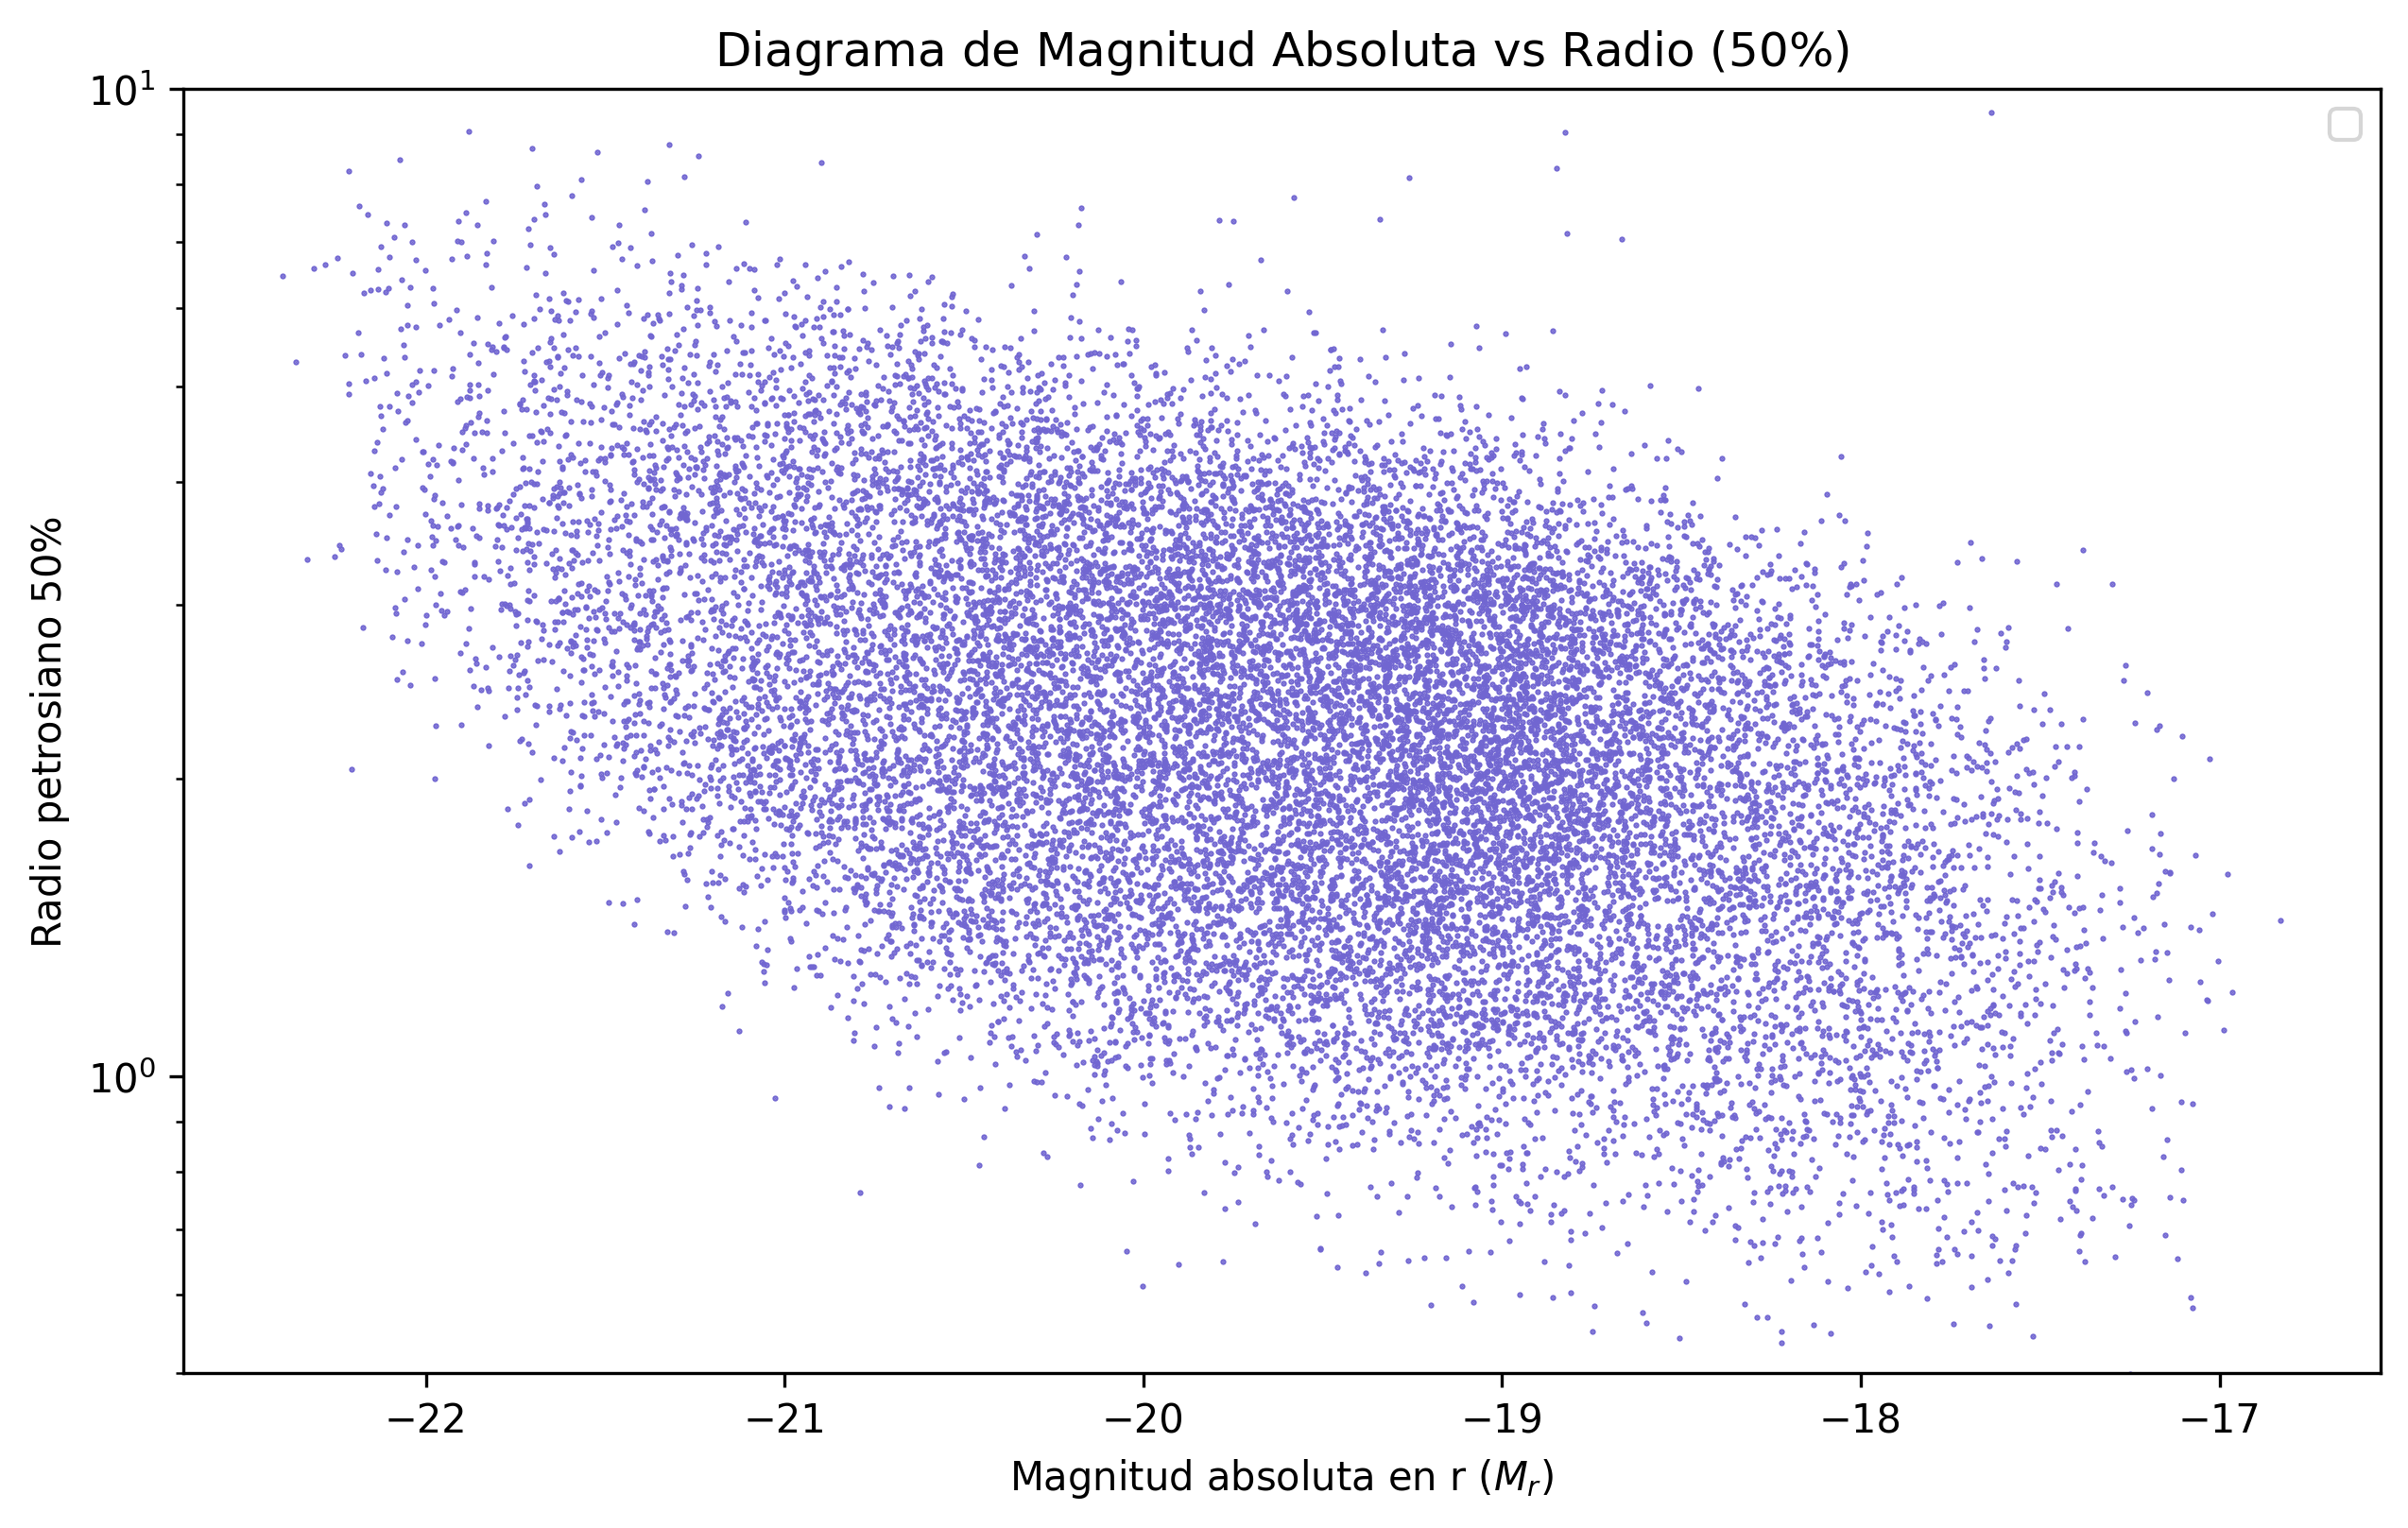
\includegraphics[width=\linewidth]{mabs_vs_r50.png}
    \caption{Relación tamaño vs. luminosidad para toda la muestra.}
    \label{fig:mabs_vs_r50}
\end{figure}

\begin{figure}[ht]
    \centering
    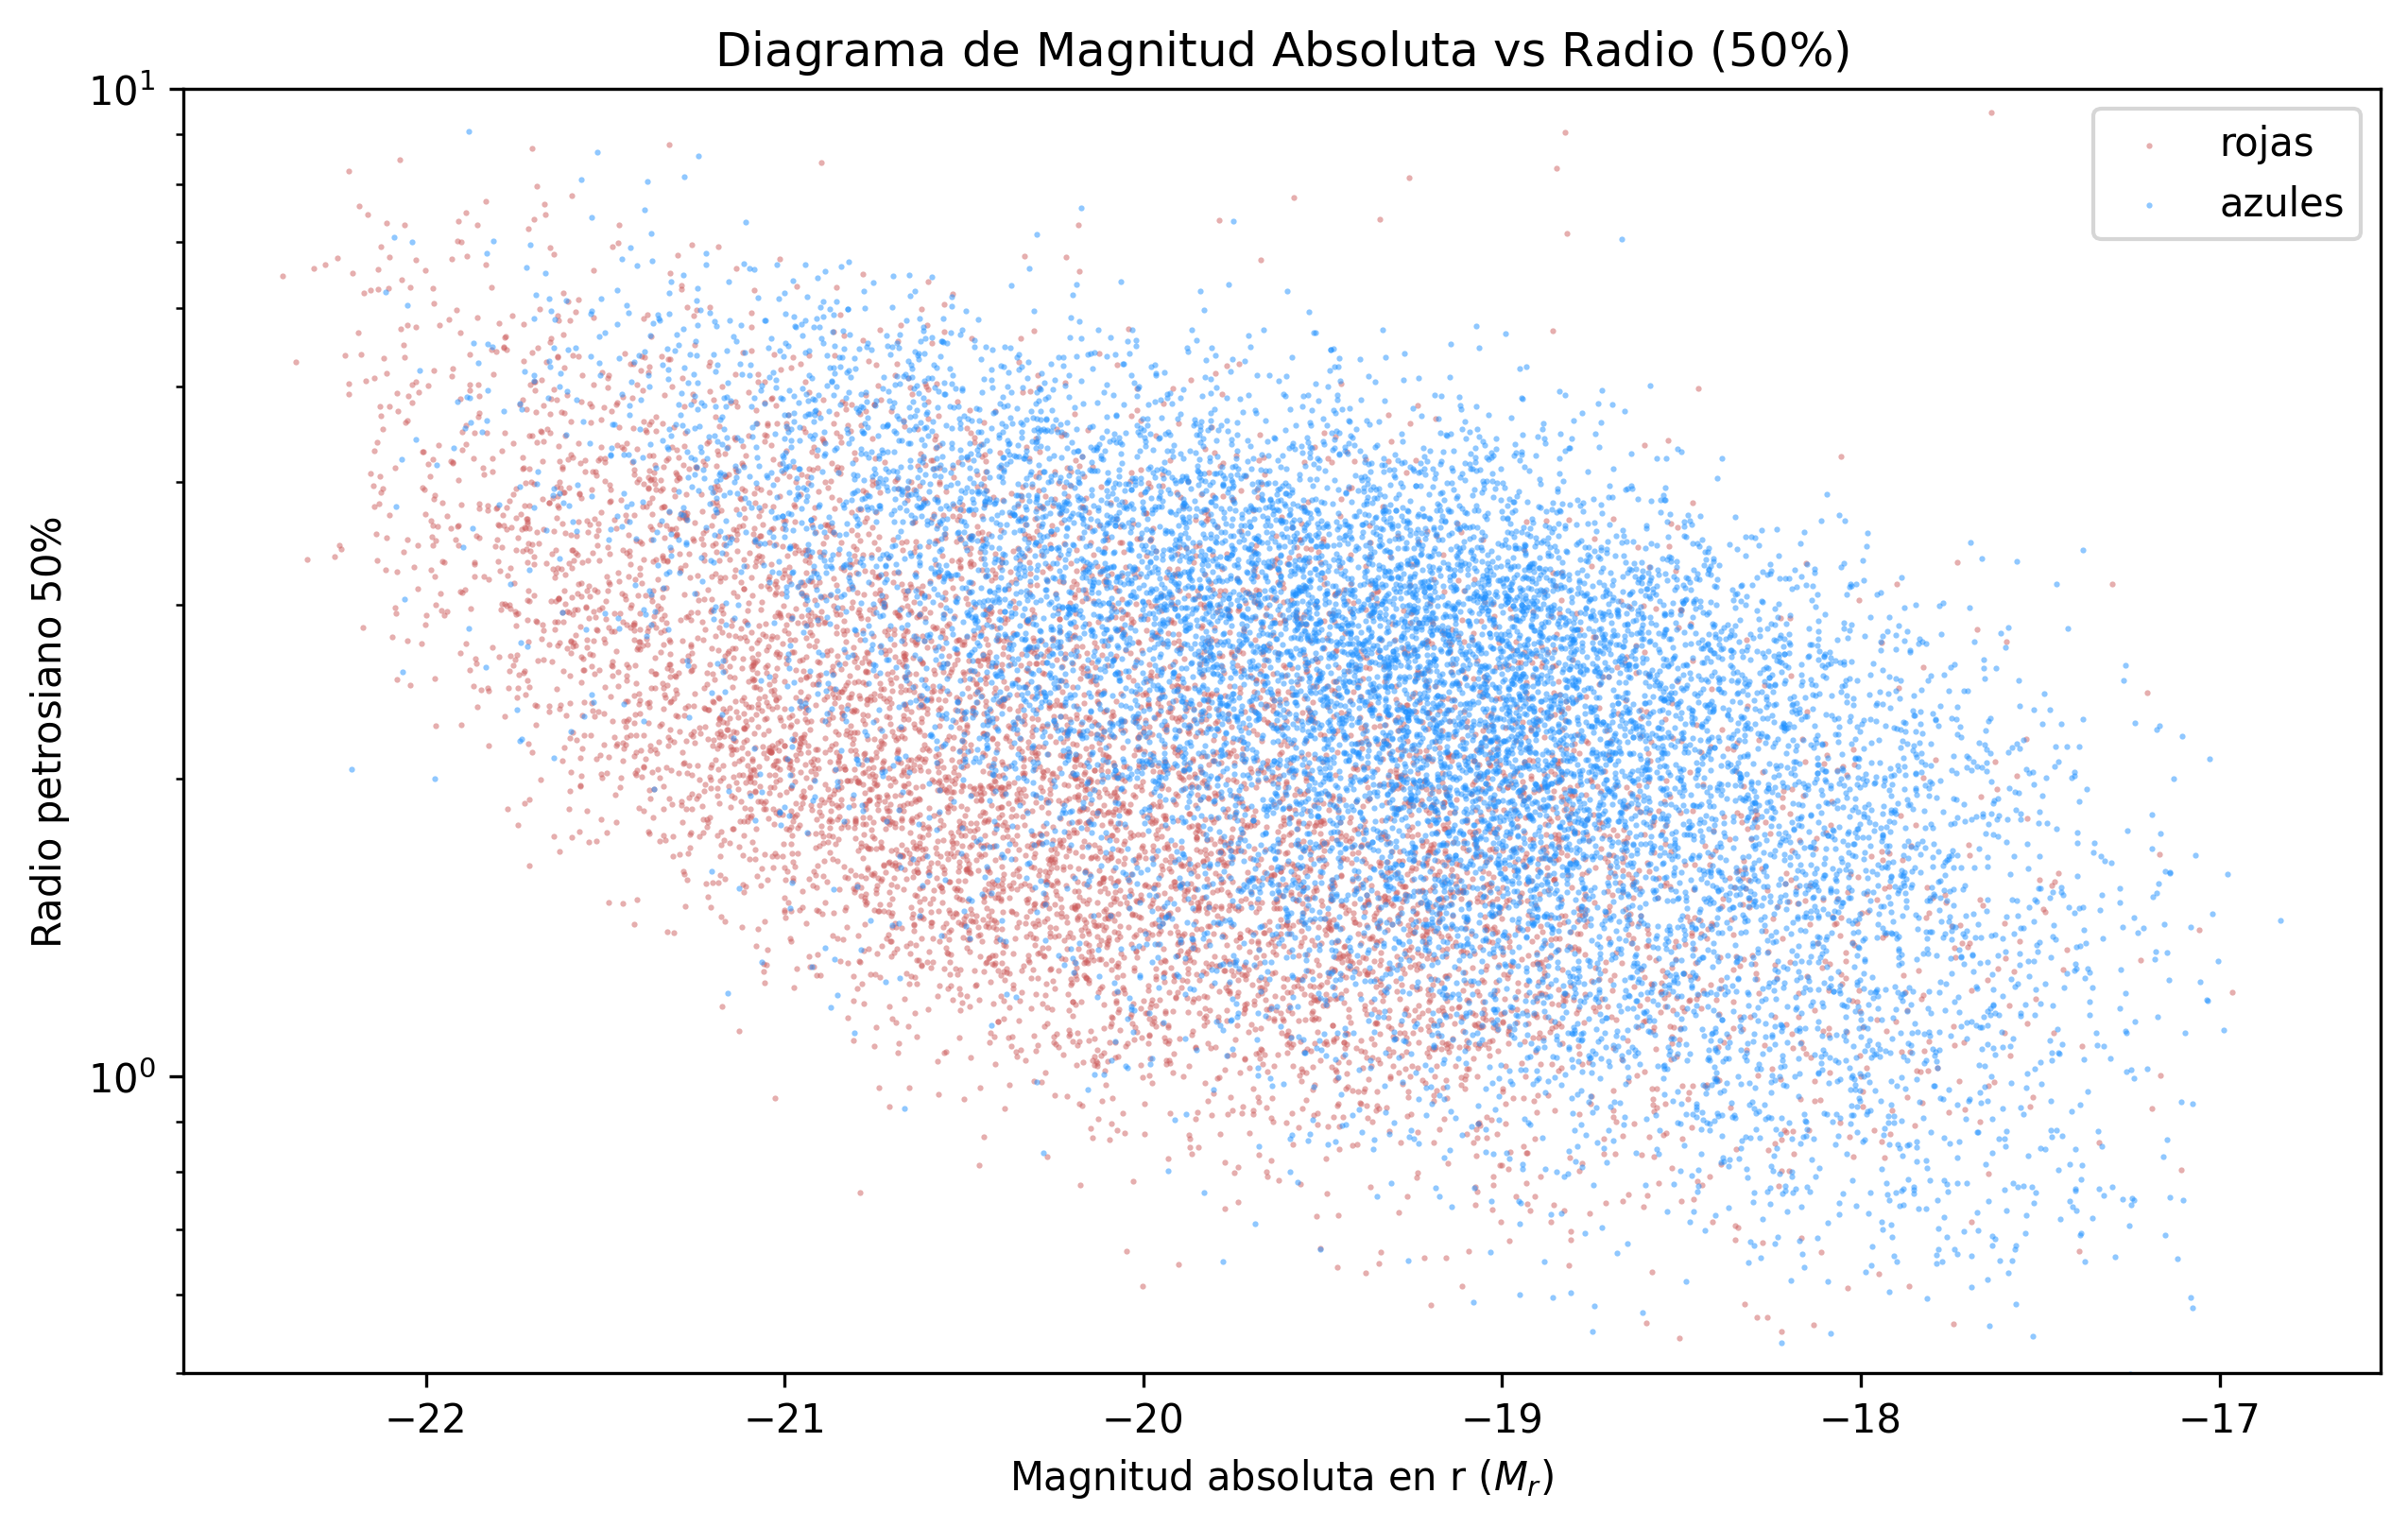
\includegraphics[width=\linewidth]{mabs_vs_r50_azulyrojo.png}
    \caption{Relación tamaño vs. luminosidad para galaxias rojas y azules.}
    \label{fig:mabs_vs_r50_rojoyazul}
\end{figure}

\begin{figure}[ht]
    \centering
    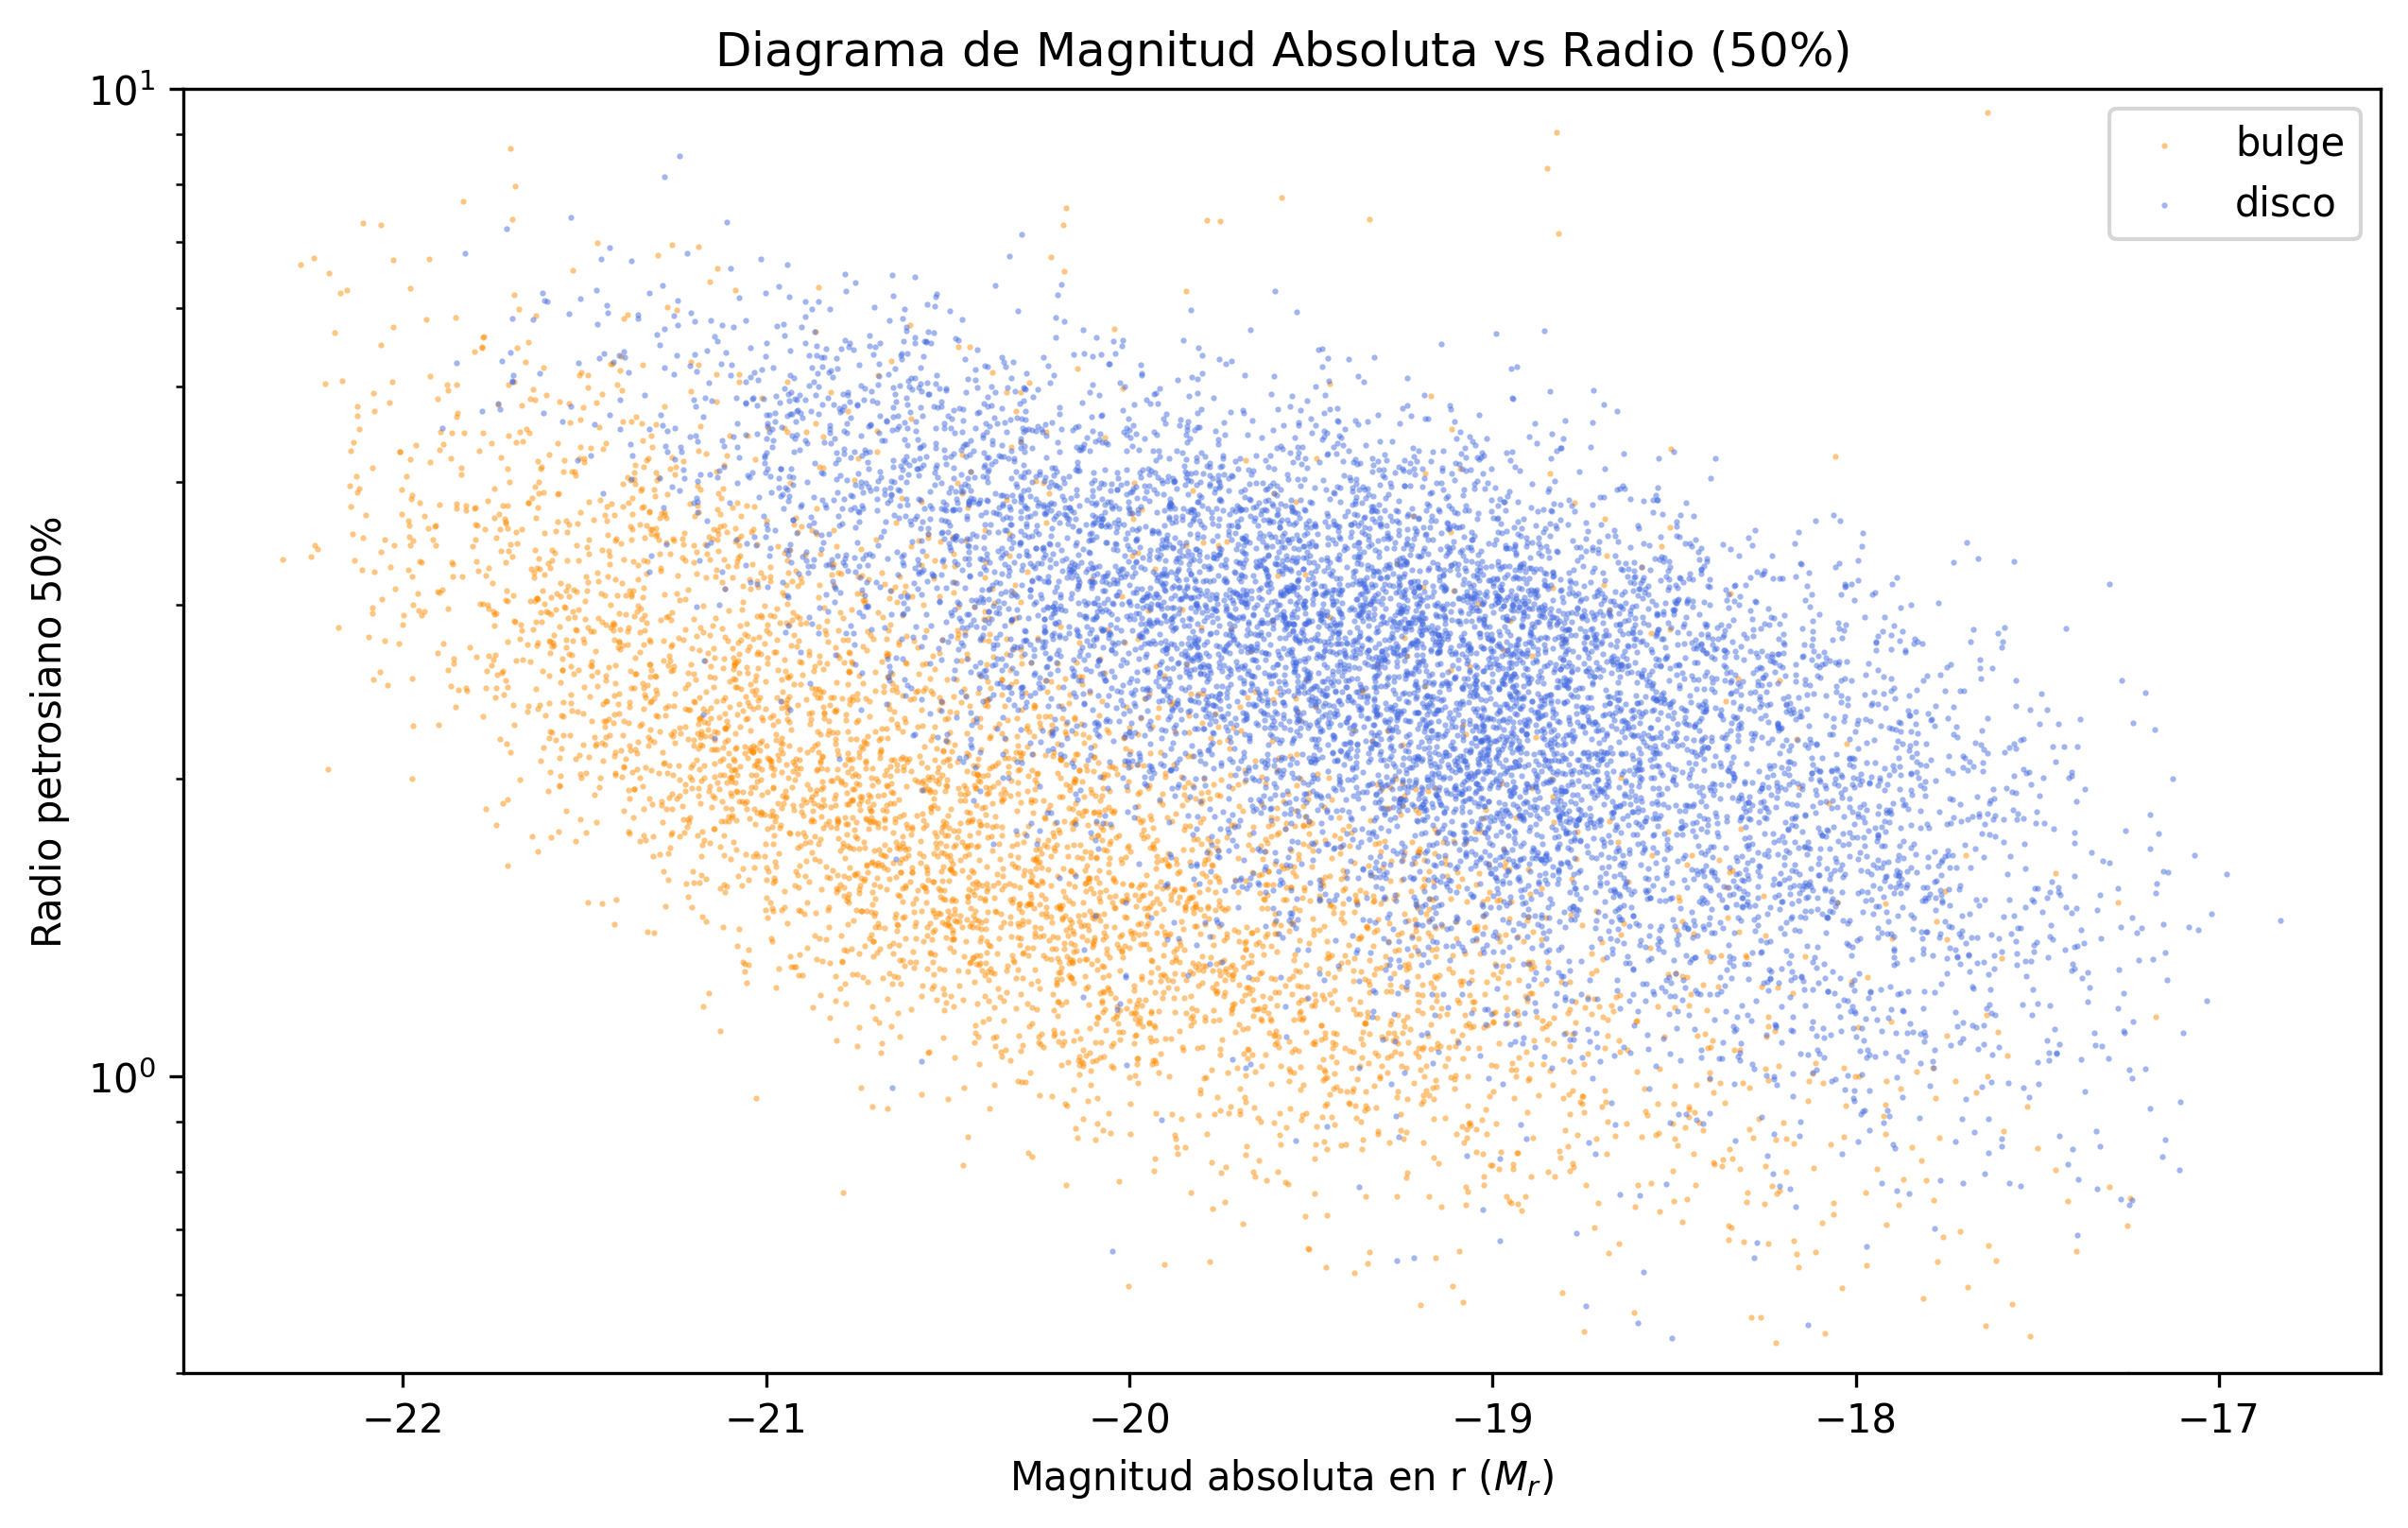
\includegraphics[width=\linewidth]{mabs_vs_r50_bulgeydisco.png}
    \caption{Relación tamaño vs. luminosidad según predominio de bulbo o disco.}
    \label{fig:mabs_vs_r50_bulgeydisco}
\end{figure}

\begin{figure}[ht]
    \centering
    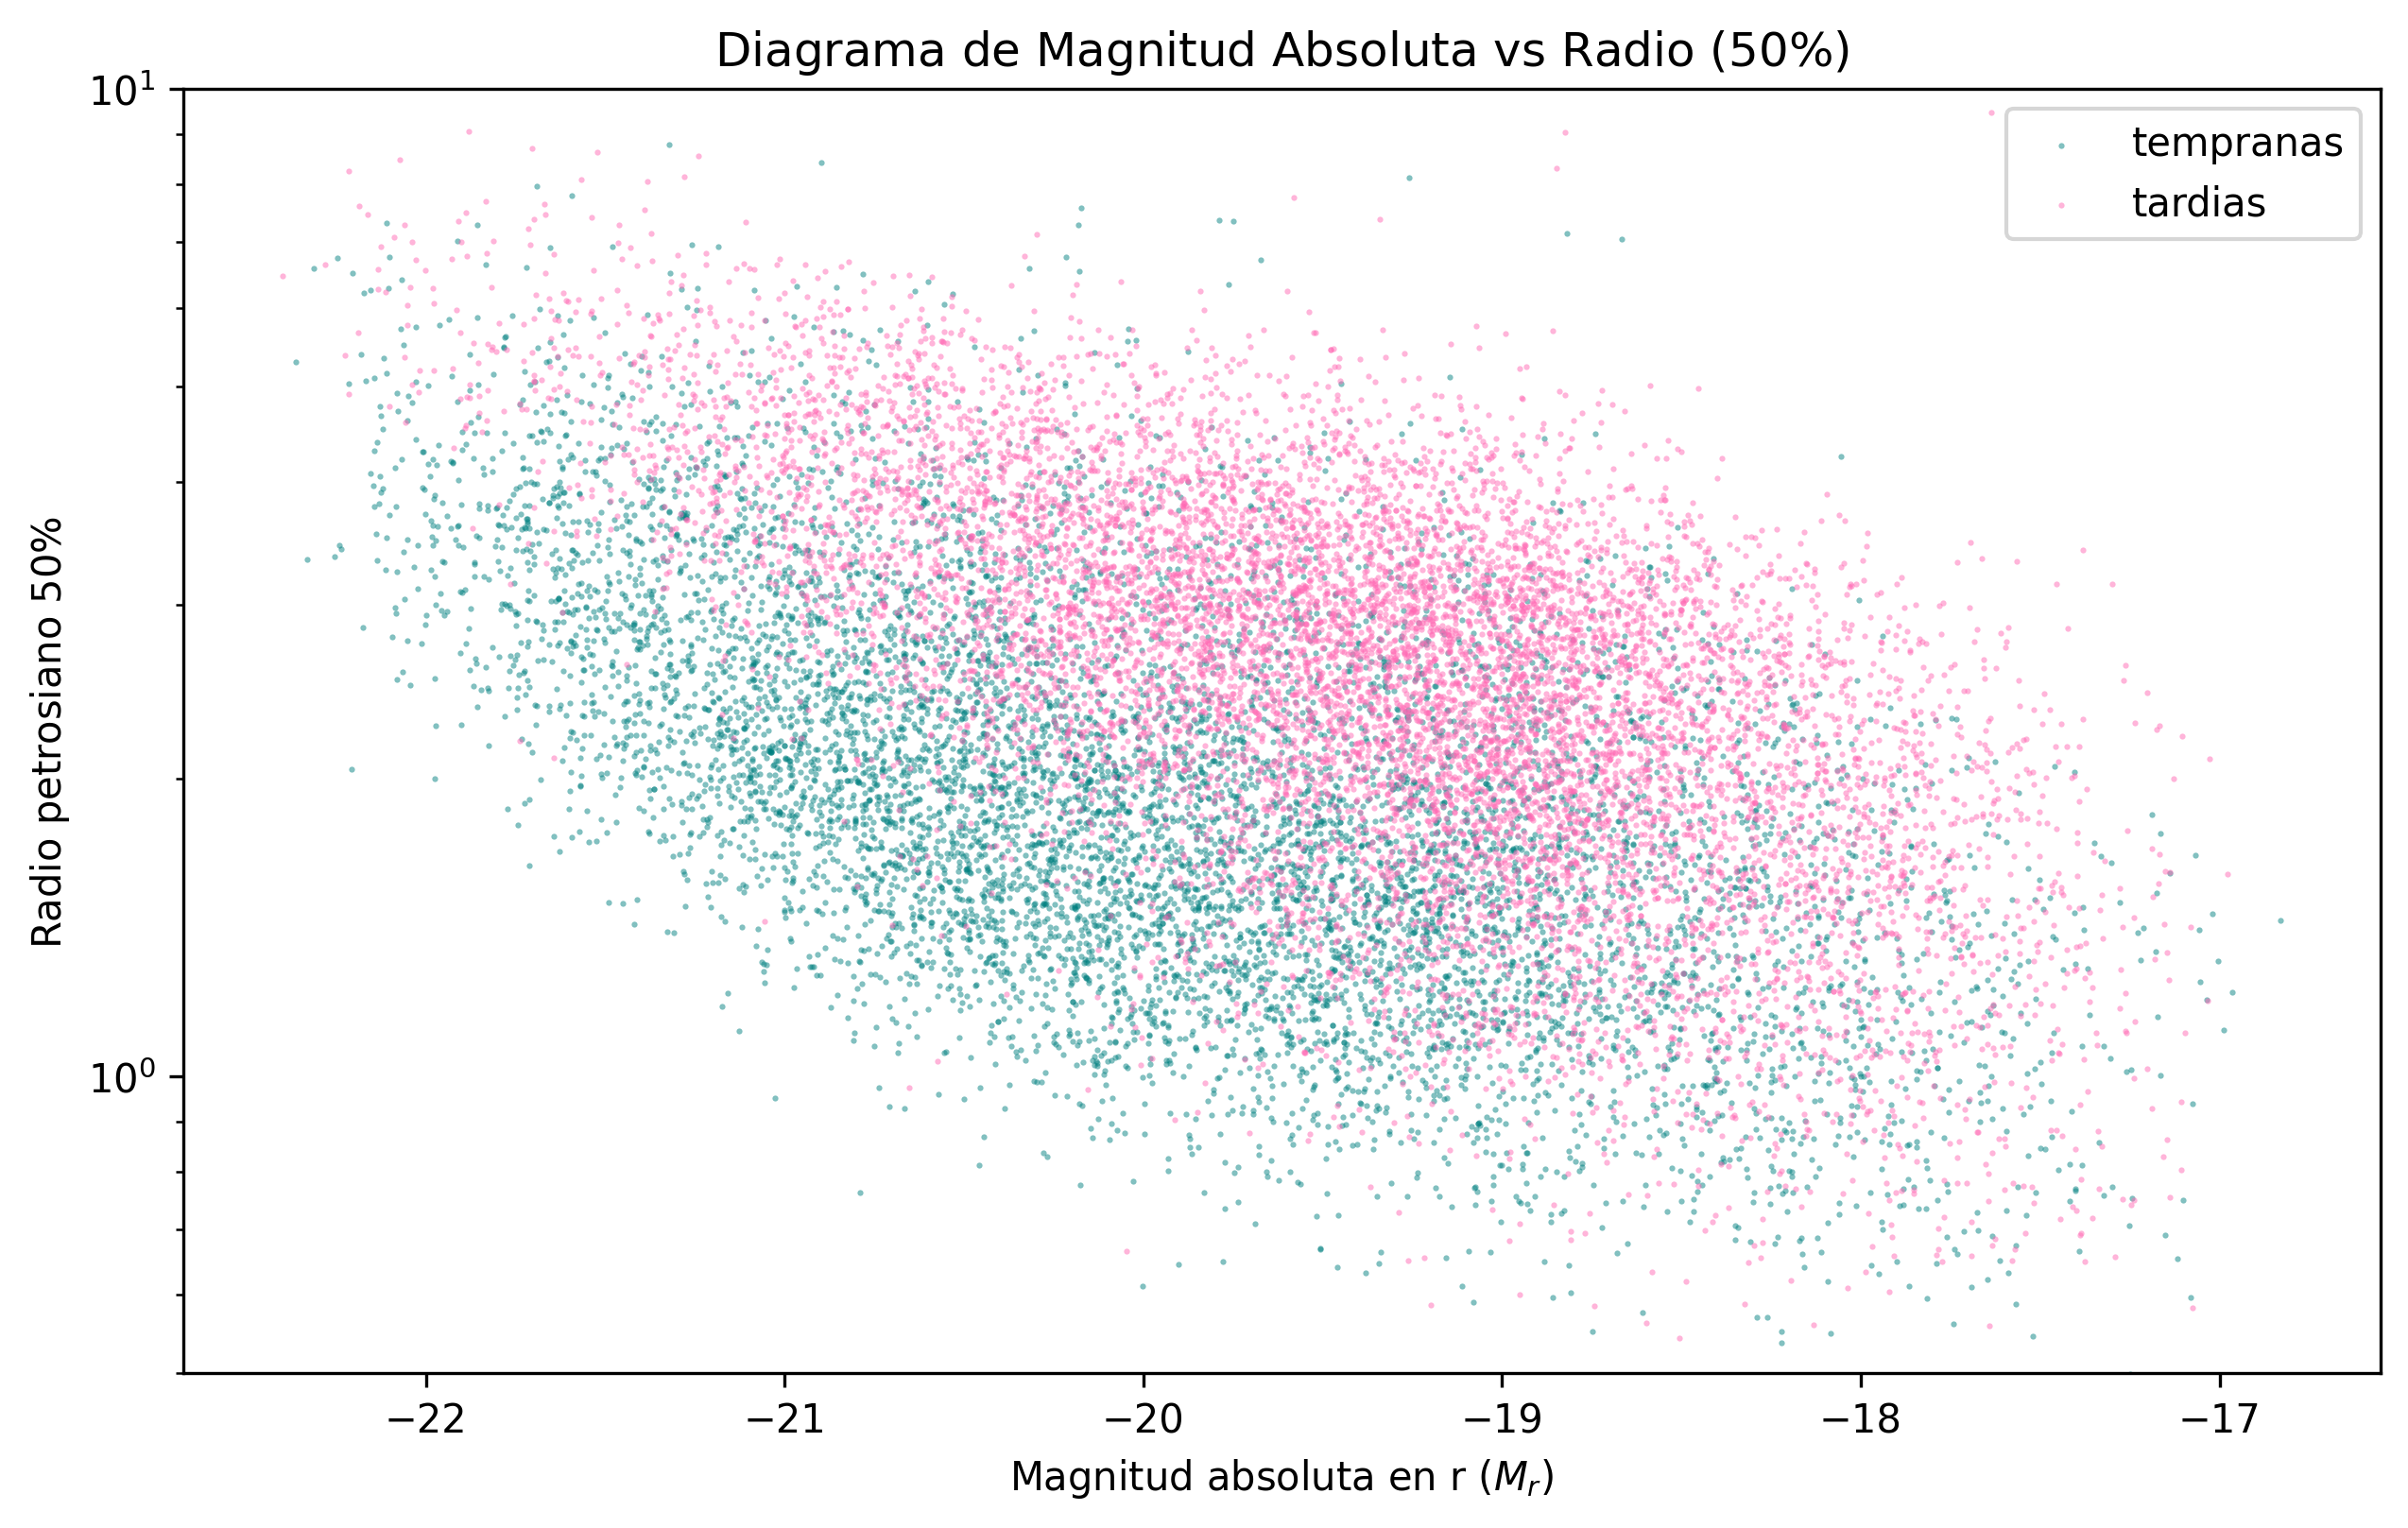
\includegraphics[width=\linewidth]{mabs_vs_r50_earlyylate.png}
    \caption{Relación tamaño vs. luminosidad para galaxias tempranas y tardías.}
    \label{fig:mabs_vs_r50_earlyylate}
\end{figure}

\subsection{Diagramas color-magnitud}

Las Figuras \ref{fig:dcm}--\ref{fig:dcm_earlyylate} muestran la nube azul y secuencia roja características. Galaxias con disco predominante se concentran en la nube azul, mientras bulgos predominan en secuencia roja.

\begin{figure}[ht]
    \centering
    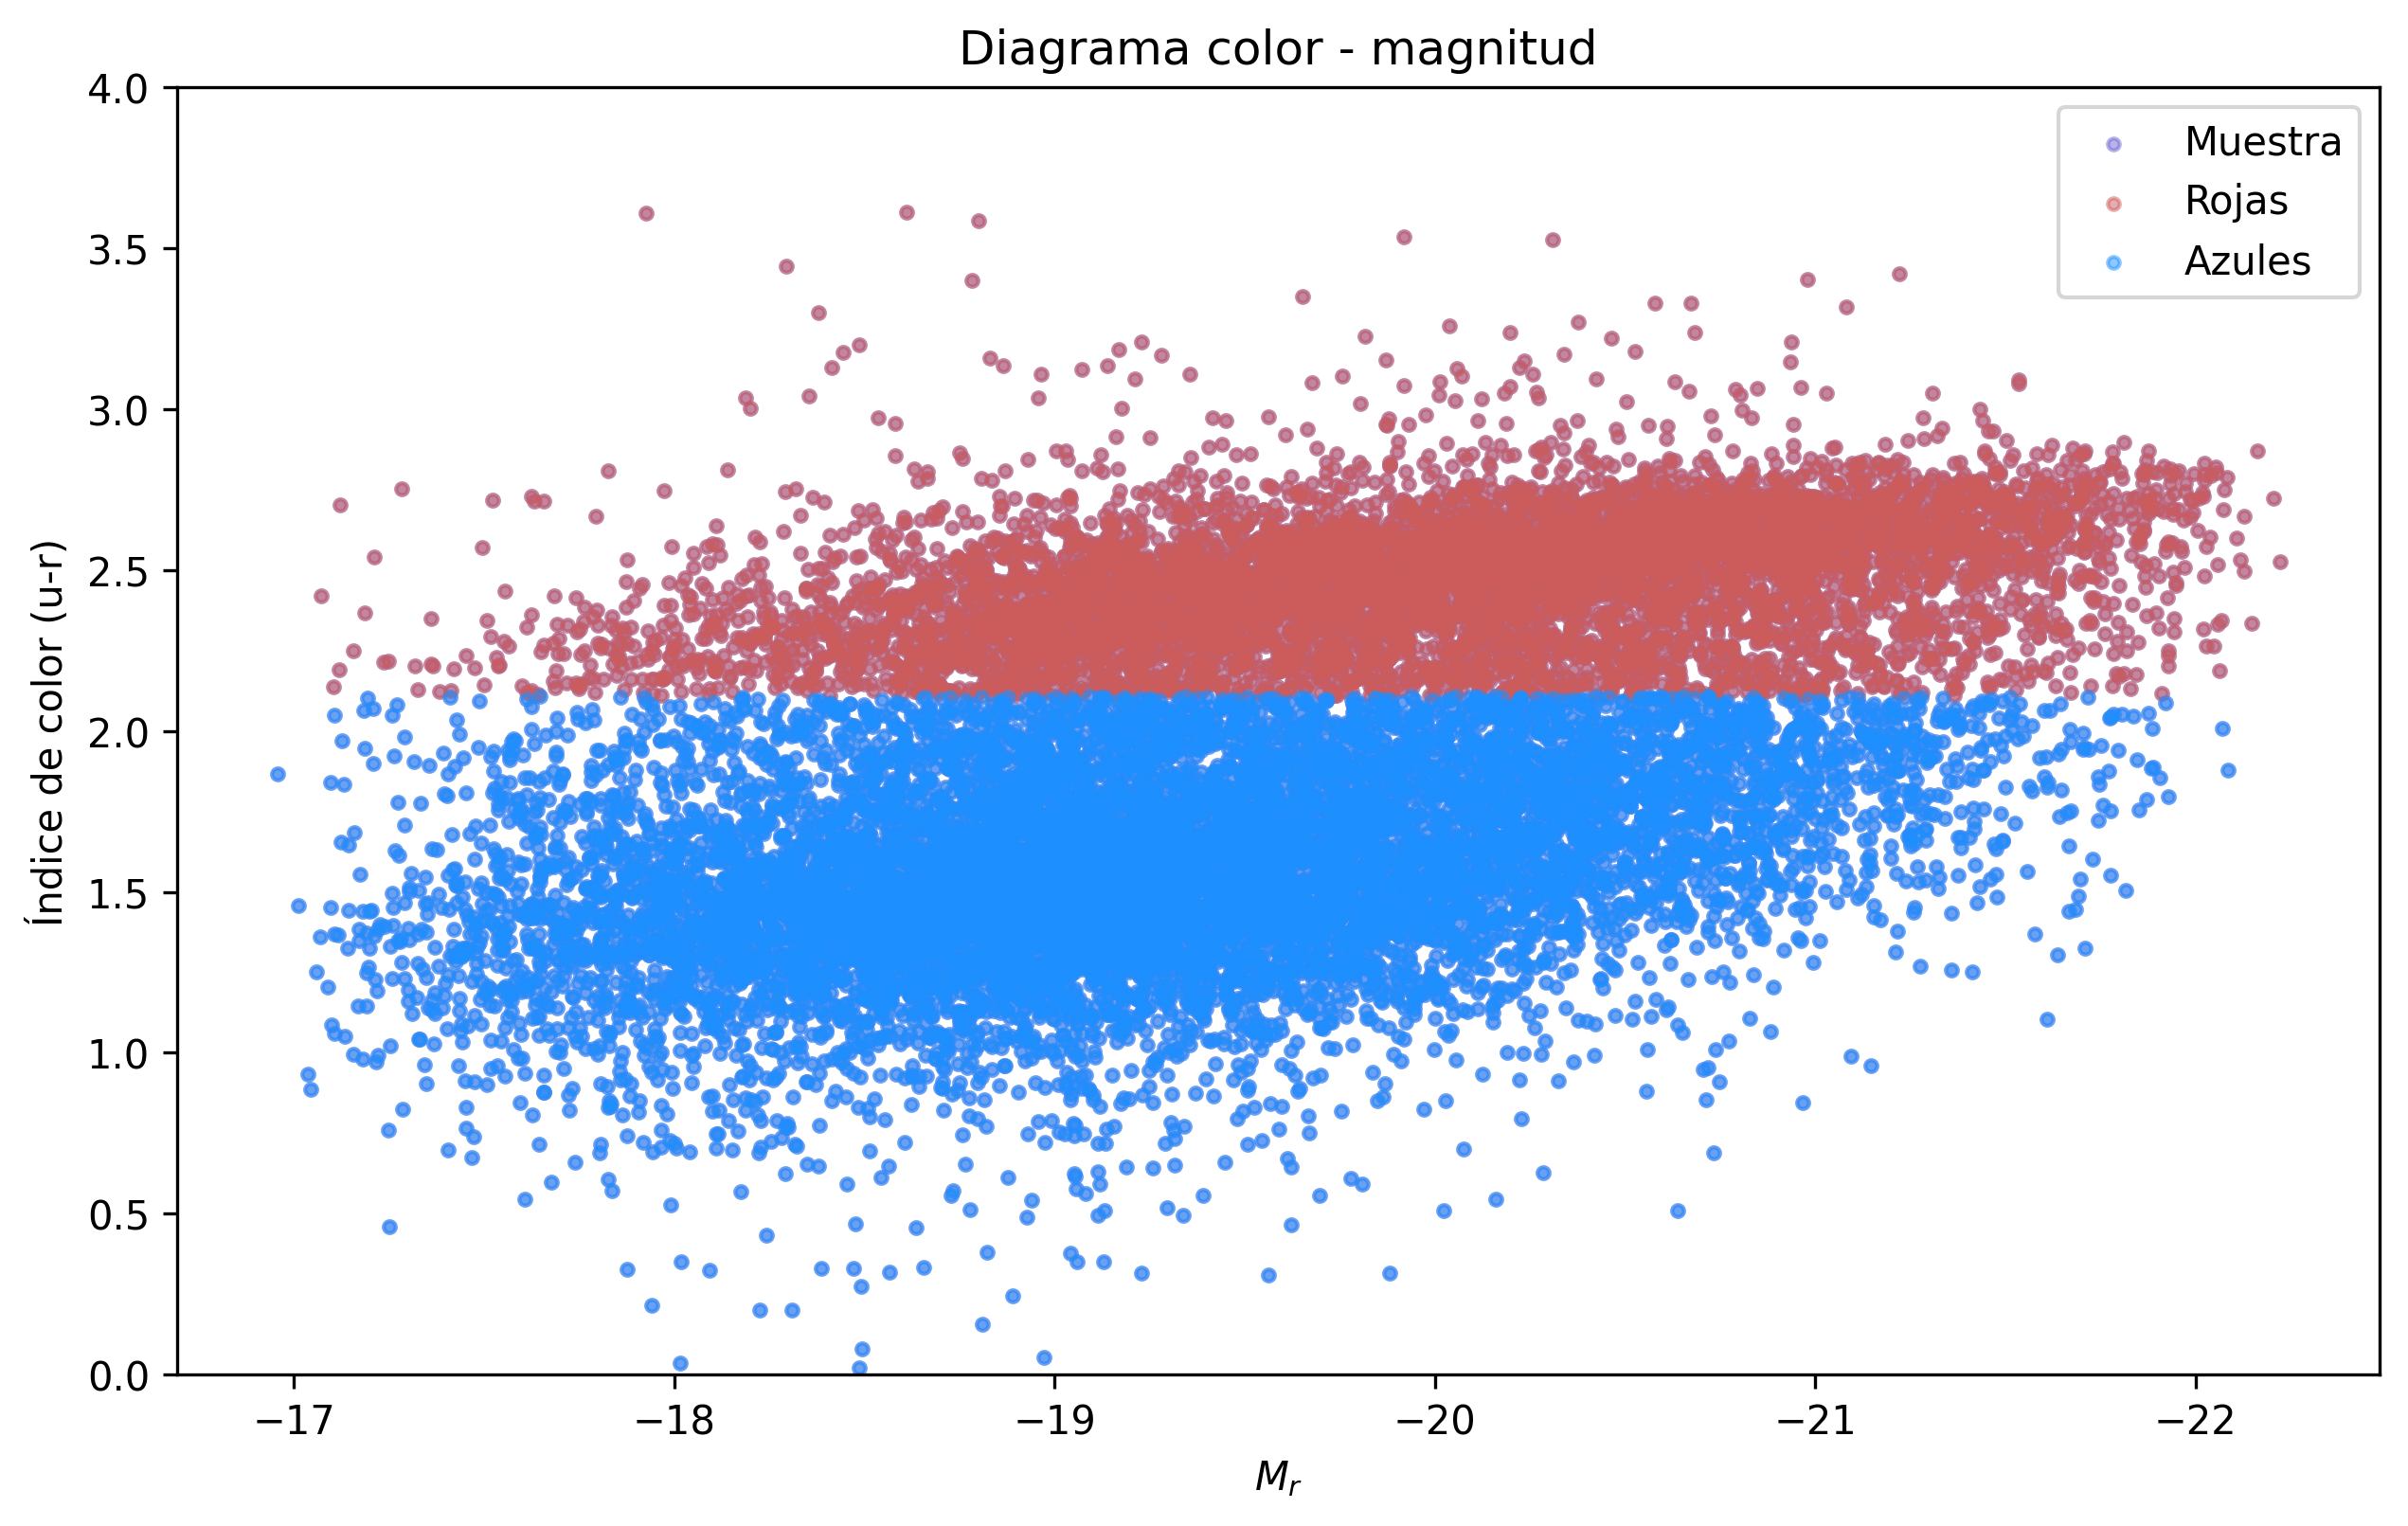
\includegraphics[width=\linewidth]{dcm_ur.png}
    \caption{Diagrama color-magnitud para galaxias rojas y azules.}
    \label{fig:dcm}
\end{figure}

\begin{figure}[ht]
    \centering
    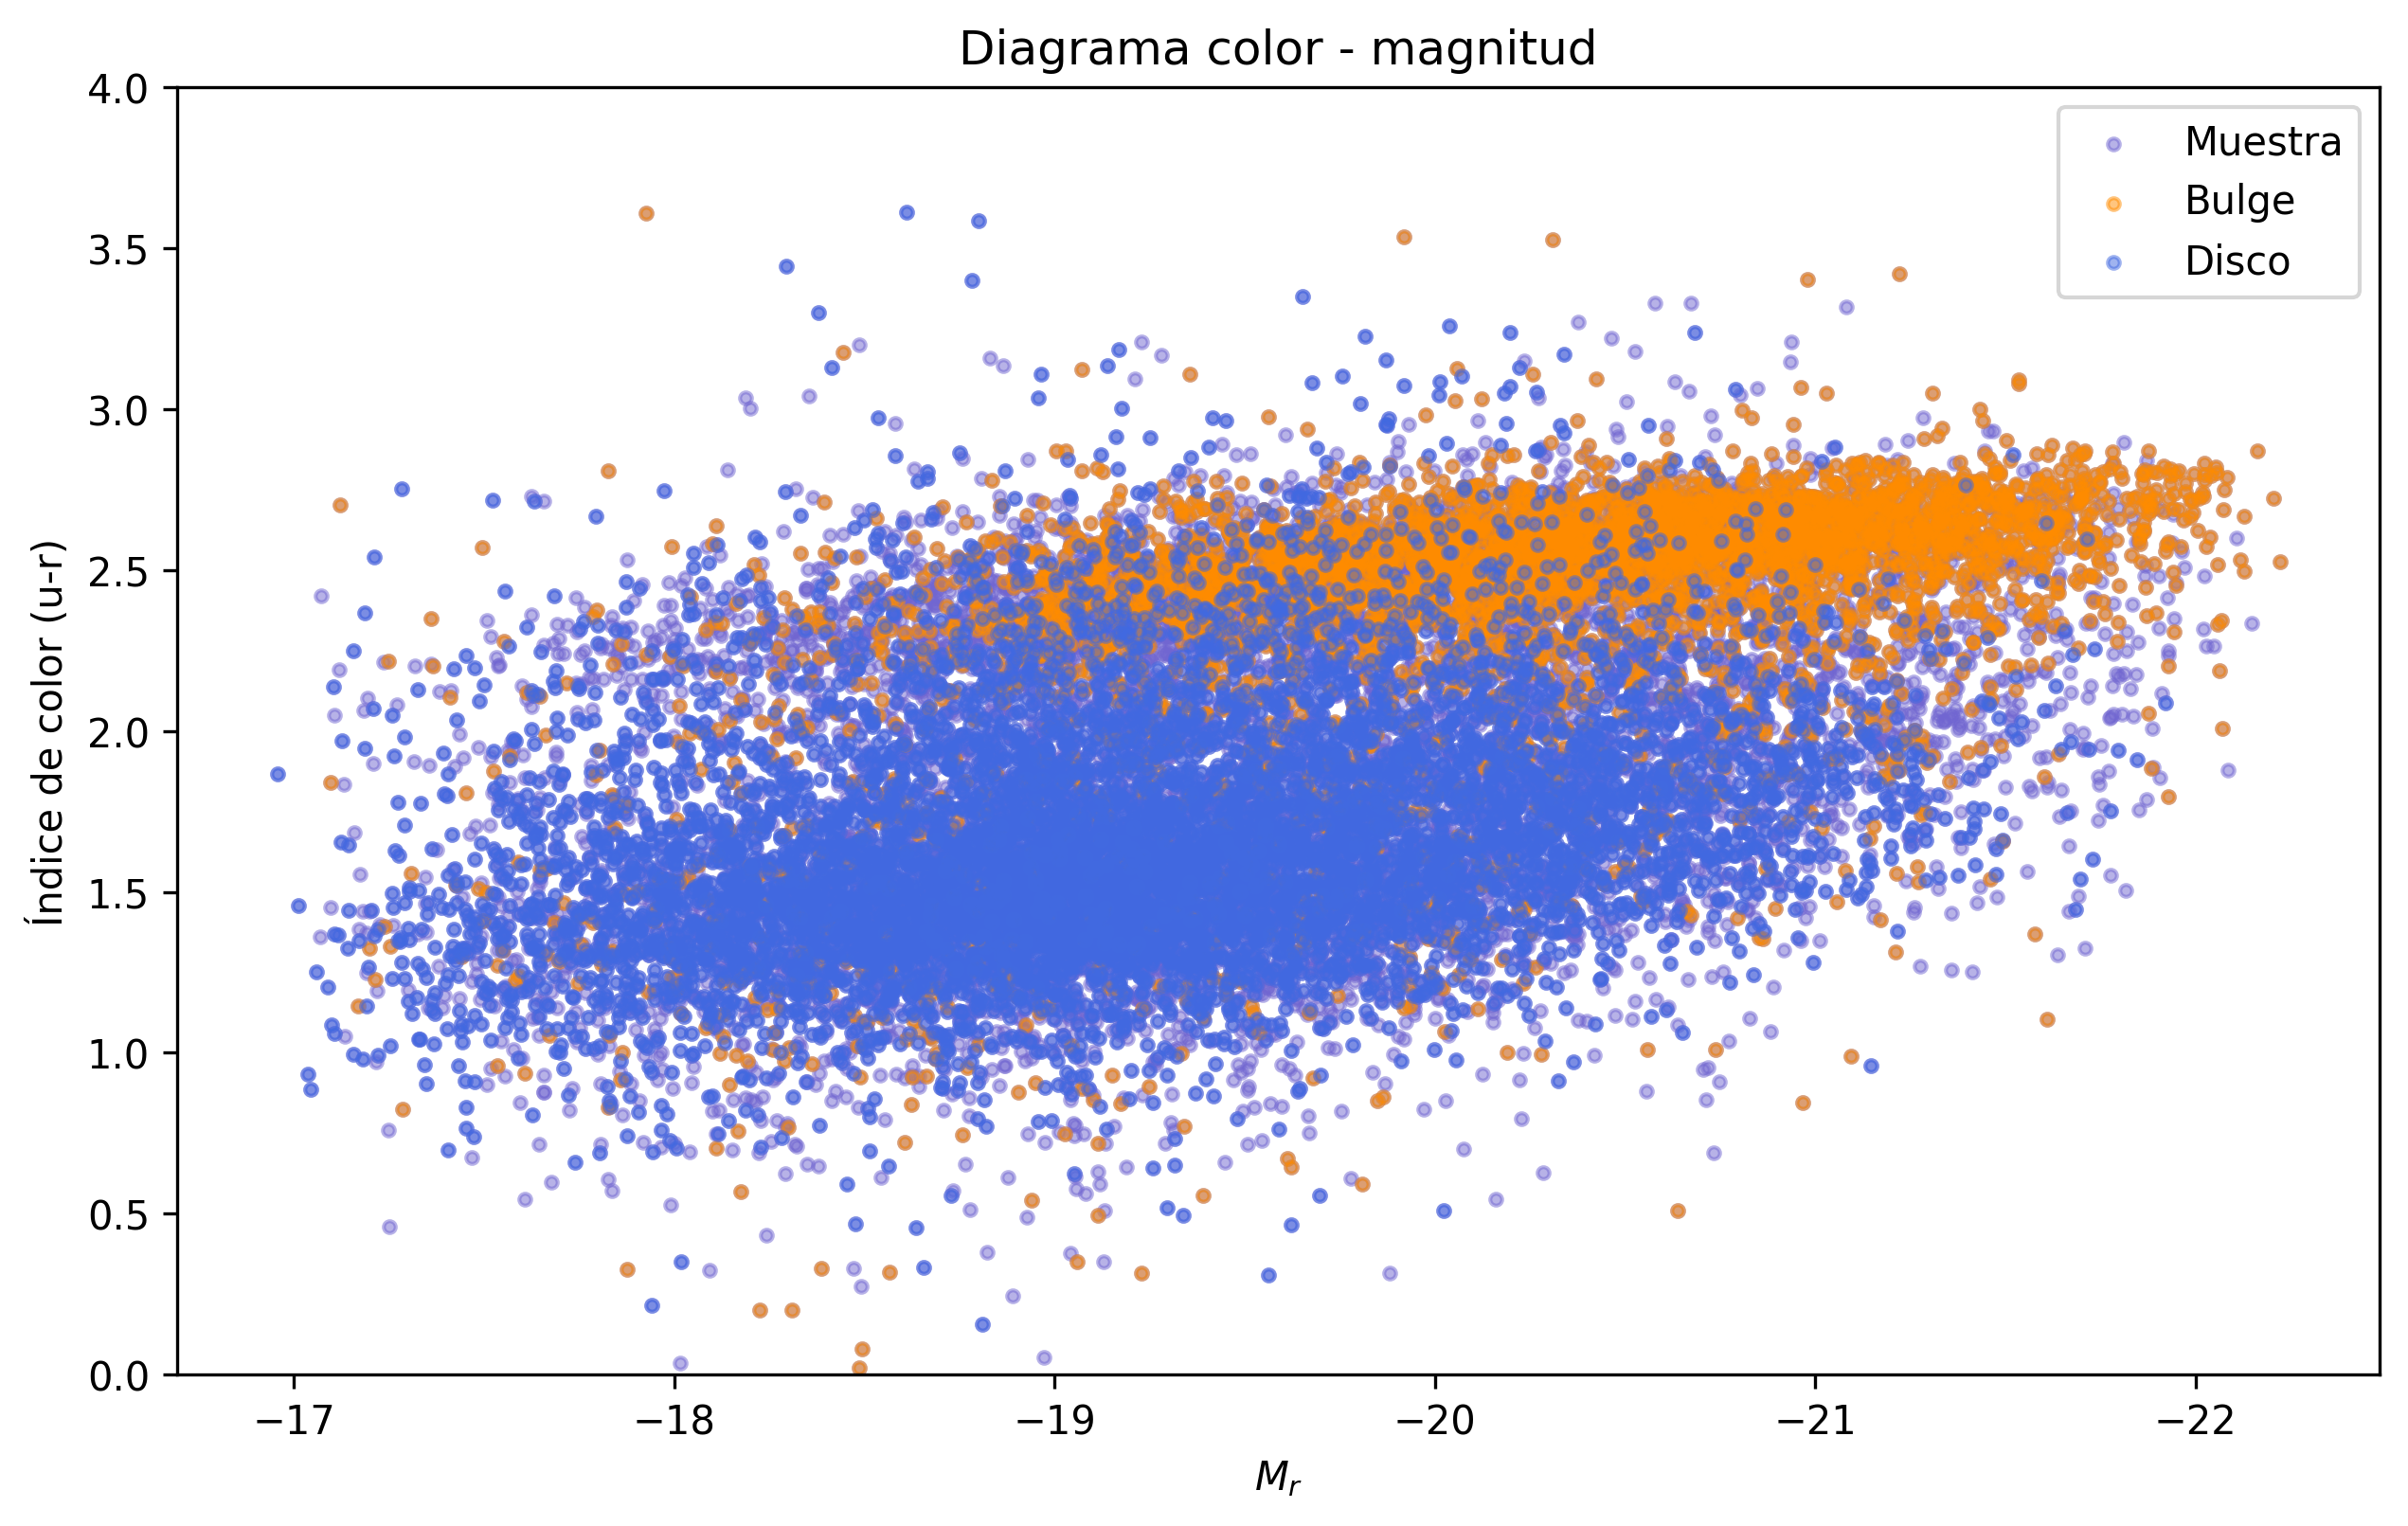
\includegraphics[width=\linewidth]{dcm_bd.png}
    \caption{Diagrama color-magnitud según predominio de bulbo o disco.}
    \label{fig:dcm_bulgeydisco}
\end{figure}

\begin{figure}[ht]
    \centering
    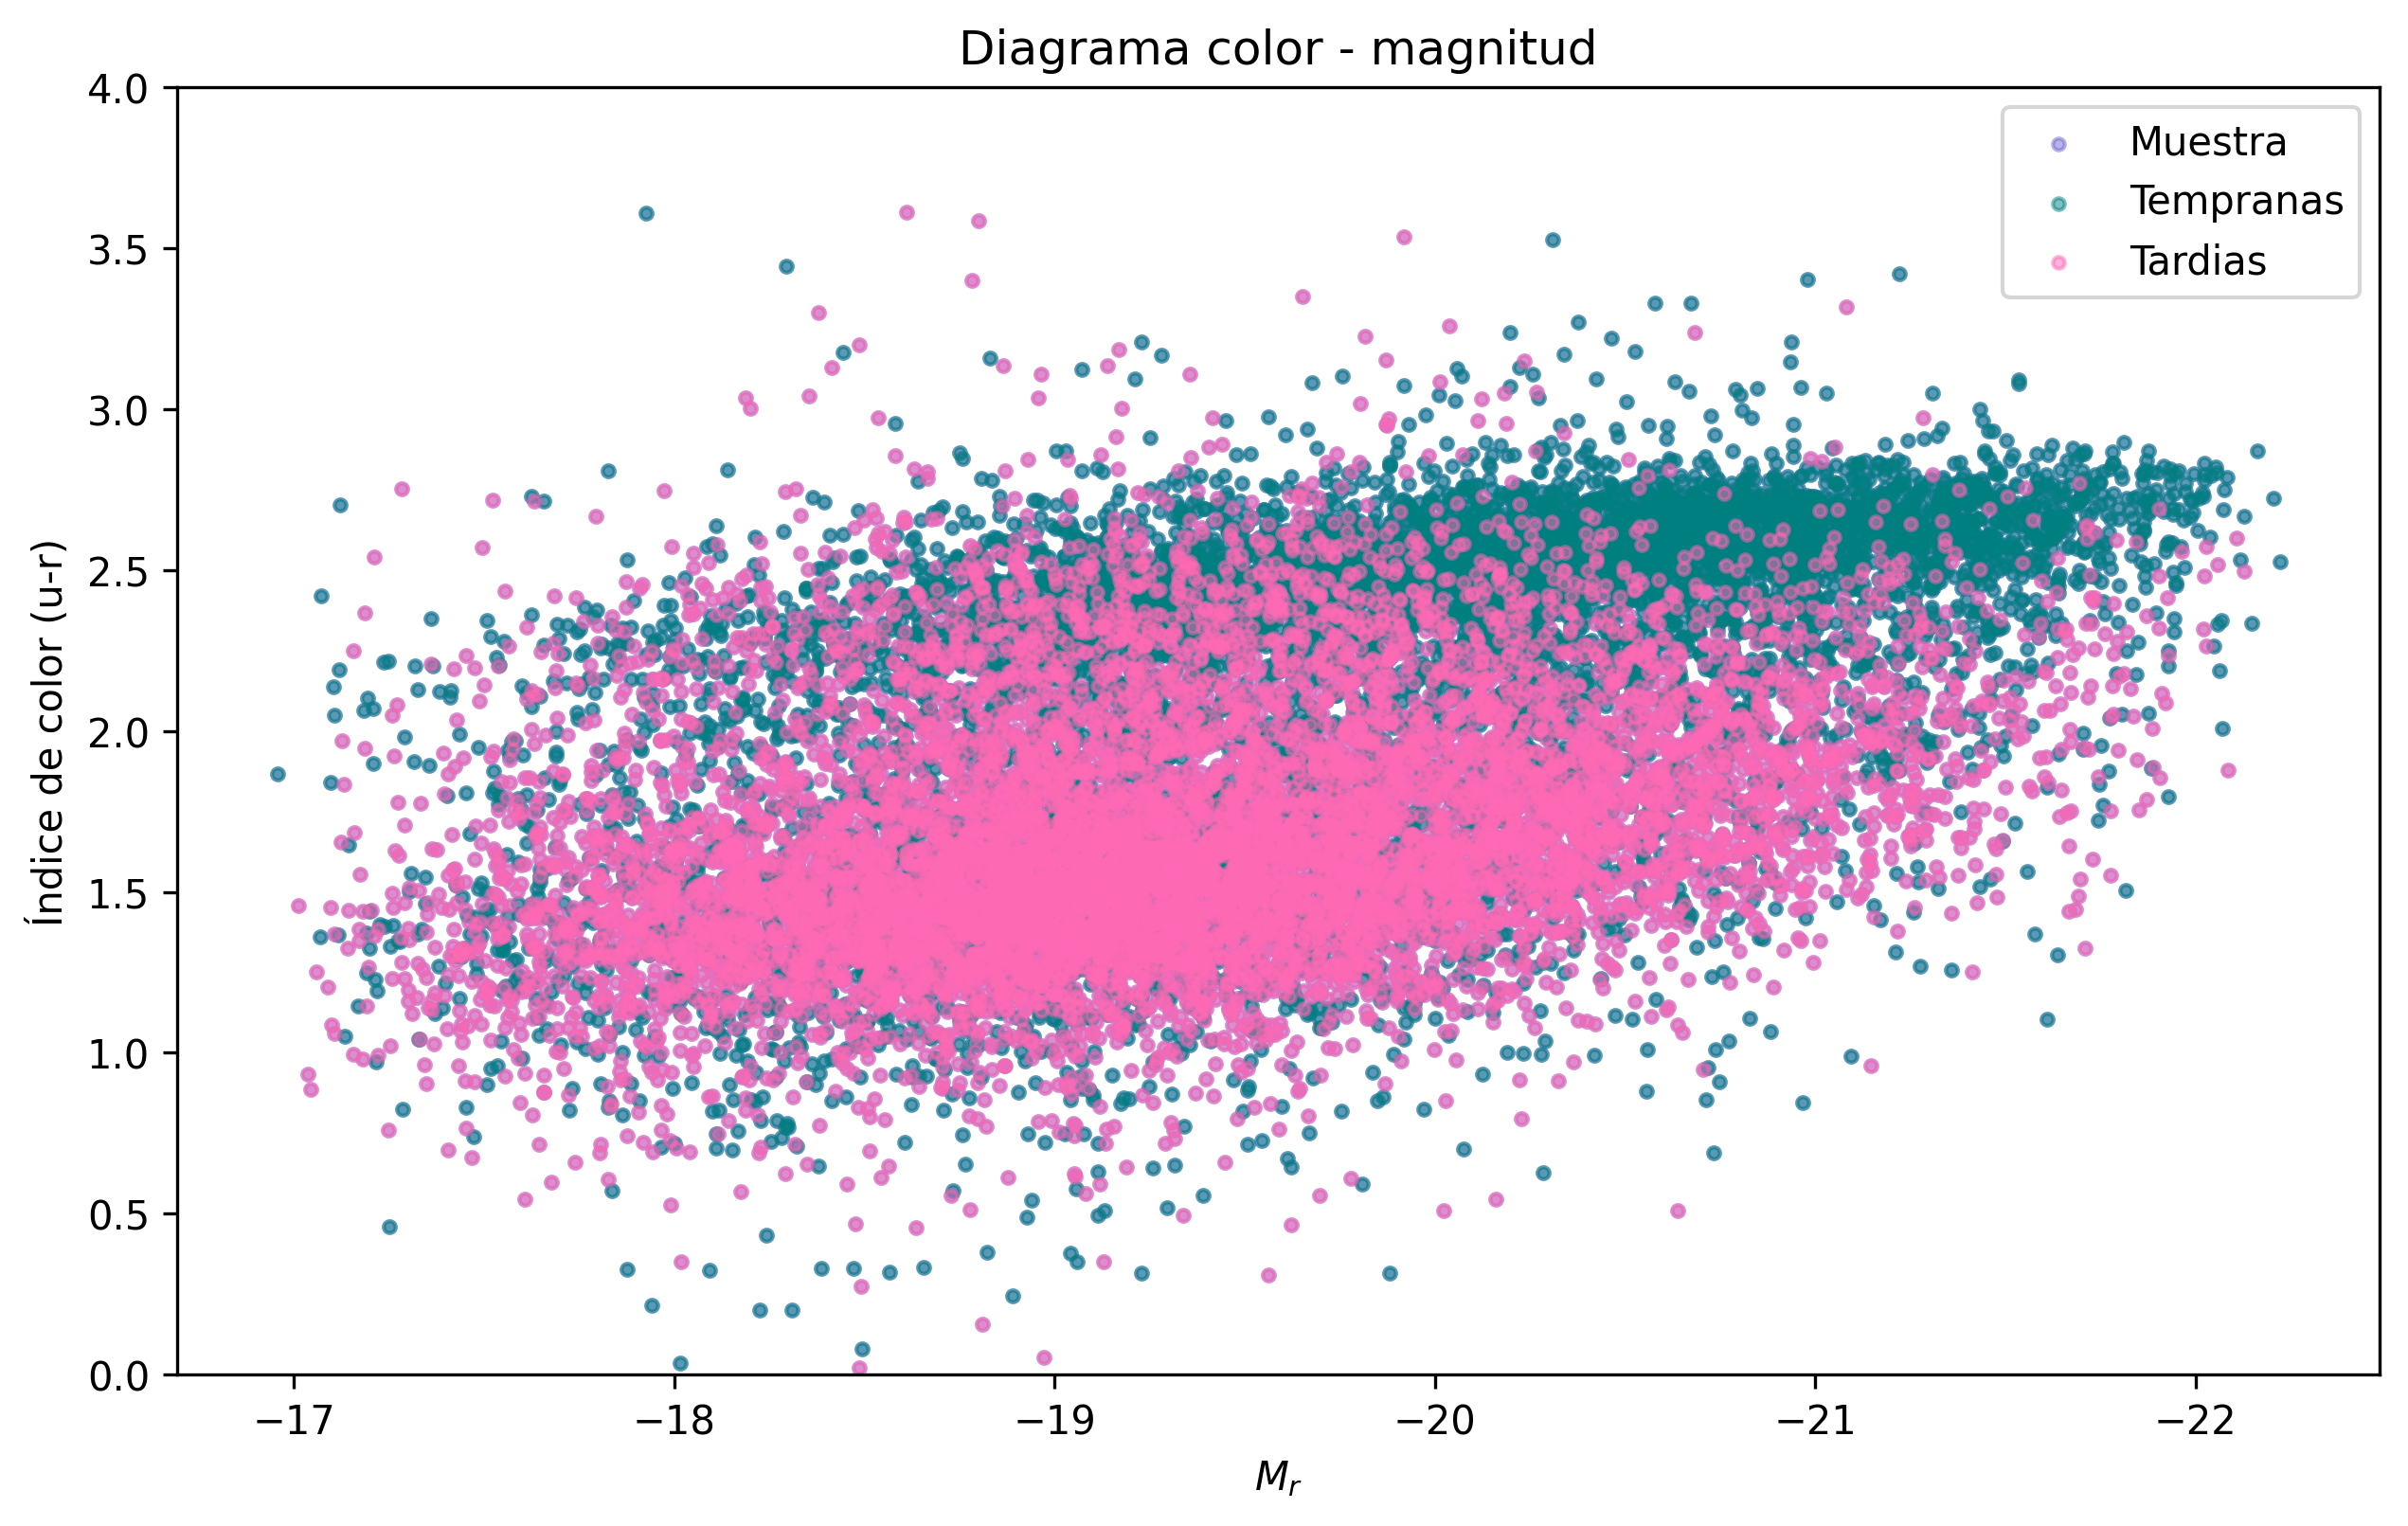
\includegraphics[width=\linewidth]{dcm_el.png}
    \caption{Diagrama color-magnitud para galaxias tempranas y tardías.}
    \label{fig:dcm_earlyylate}
\end{figure}

\section{Conclusiones}

El análisis revela correlaciones significativas entre parámetros morfológicos y propiedades fotométricas:

\begin{itemize}
    \item La muestra presenta bimodalidad en índices de color, consistente con literatura
    \item Existe correlación entre concentración y parámetro fracDeV
    \item Las relaciones tamaño-luminosidad muestran dependencias con tipo morfológico
    \item Los diagramas color-magnitud confirman la secuencia roja y nube azul
    \item Los parámetros de SDSS permiten clasificación morfológica robusta
\end{itemize}

Estos resultados demuestran la utilidad de los catálogos modernos para estudios estadísticos de poblaciones galácticas.

\bibliographystyle{plainnat}
\bibliography{bibliografia}

\end{document}